% !TEX root = ./../main.tex
\chapter{Molecular description of the process}
%Introduzione a seguito dei risultati con la metadinamica: run unbiased con PW striped, random11, random 12 e POPC
In view of the results obtained with metadynamics, shown in the previous chapter, and in order to try to see the anchoring process to spontaneously occur, we decide to perform unbiased runs starting from the hydrophobic state for all the anionic \ac{AuNP} configurations: the striped (\ac{MUS}:\ac{OT} $1$:$1$), the random (\ac{MUS}:\ac{OT} $1$:$1$) and the random (\ac{MUS}:\ac{OT} $2$:$1$), with both \ac{PME} and \ac{PW} model. This runs are suitable to get some useful information about the molecular processes involved and about the hydrophobic state with a more realistic \ac{CG} description.

Unfortunately, with ten of microseconds for each configurations, we have not seen any anchoring process. This confirm, in accordance with the atomistic model and the metadynamics results, the increase of the energy barrier respect to the standard \martini model and the slowdown of the dynamics of the system. Despite this, the unbiased runs are useful in order for a comparison with the metadynamics runs to be made. In particular we can compare some interesting molecular phenomena that we have see in metadynamics runs such as: the dragging of the water bead inside the hydrophobic region of the membrane by the charged bead during the anchoring process; the choline group bead of the entrance leaflet dragged inside the hydrophobic region by the charged bead during the anchoring process and the engulfment effect of the opposite leaflet during the dis--anchor process. Moreover, comparing the results of the hydrophobic state only, we can get some information about the destructiveness of the metadynamics and if and how the bilayer properties change. 


\section{Water dragging}
\label{sec:WDragging}
%Trascinamento delle PW nelle varie salse
In order to study if there is an increase of water beads inside the hydrophobic region of the bilayer during the anchoring process as the model accuracy increase, I calculate the number contacts with water bead within $0.6$~nm from charged bead in function of the time. Then, obtaining the $z$ component of the distance of the charged bead from the bilayer \ac{COM} in function of the time, since the time step is set to be equal to $1$~ns for both, I can correlate the two quantities. The obtained data is binned with a bin width of $0.08$~nm and the total number of counts per bin is normalized with the number of the bin entries. The results is the plot shown in figure~(\ref{fig:WContact}). As explained previously, $z=0$ is the center of the bilayer, $z<0$ corresponds to the entrance leaflet and the \ac{NP} is in the hydrophobic state; for $z>0$, instead, the \ac{NP} is approaching the anchored state and the charged bead is in the opposite leaflet. In particular, in figure~(\ref{fig:WContact}a) is shown a comparison between different \ac{CG} \martini models: the standard, with \ac{PME} alone and with both \ac{PME} and \ac{PW}. Instead, in figure~(\ref{fig:WContact}b) is shown a comparison between the striped and the random \acp{NP} with both \ac{PME} and \ac{PW}. For the number of contacts with the \ac{PW} bead, since the ligand is negatively charged, only the contacts with the $WP$ particle of the \ac{PW} bead is considered.
%	WPatchedComparison		WRPComparison
%\newgeometry{left=2.5cm,right=2.5cm}
\begin{figure}[!ht]
	\center
	\subfloat[striped – model comparison]{
		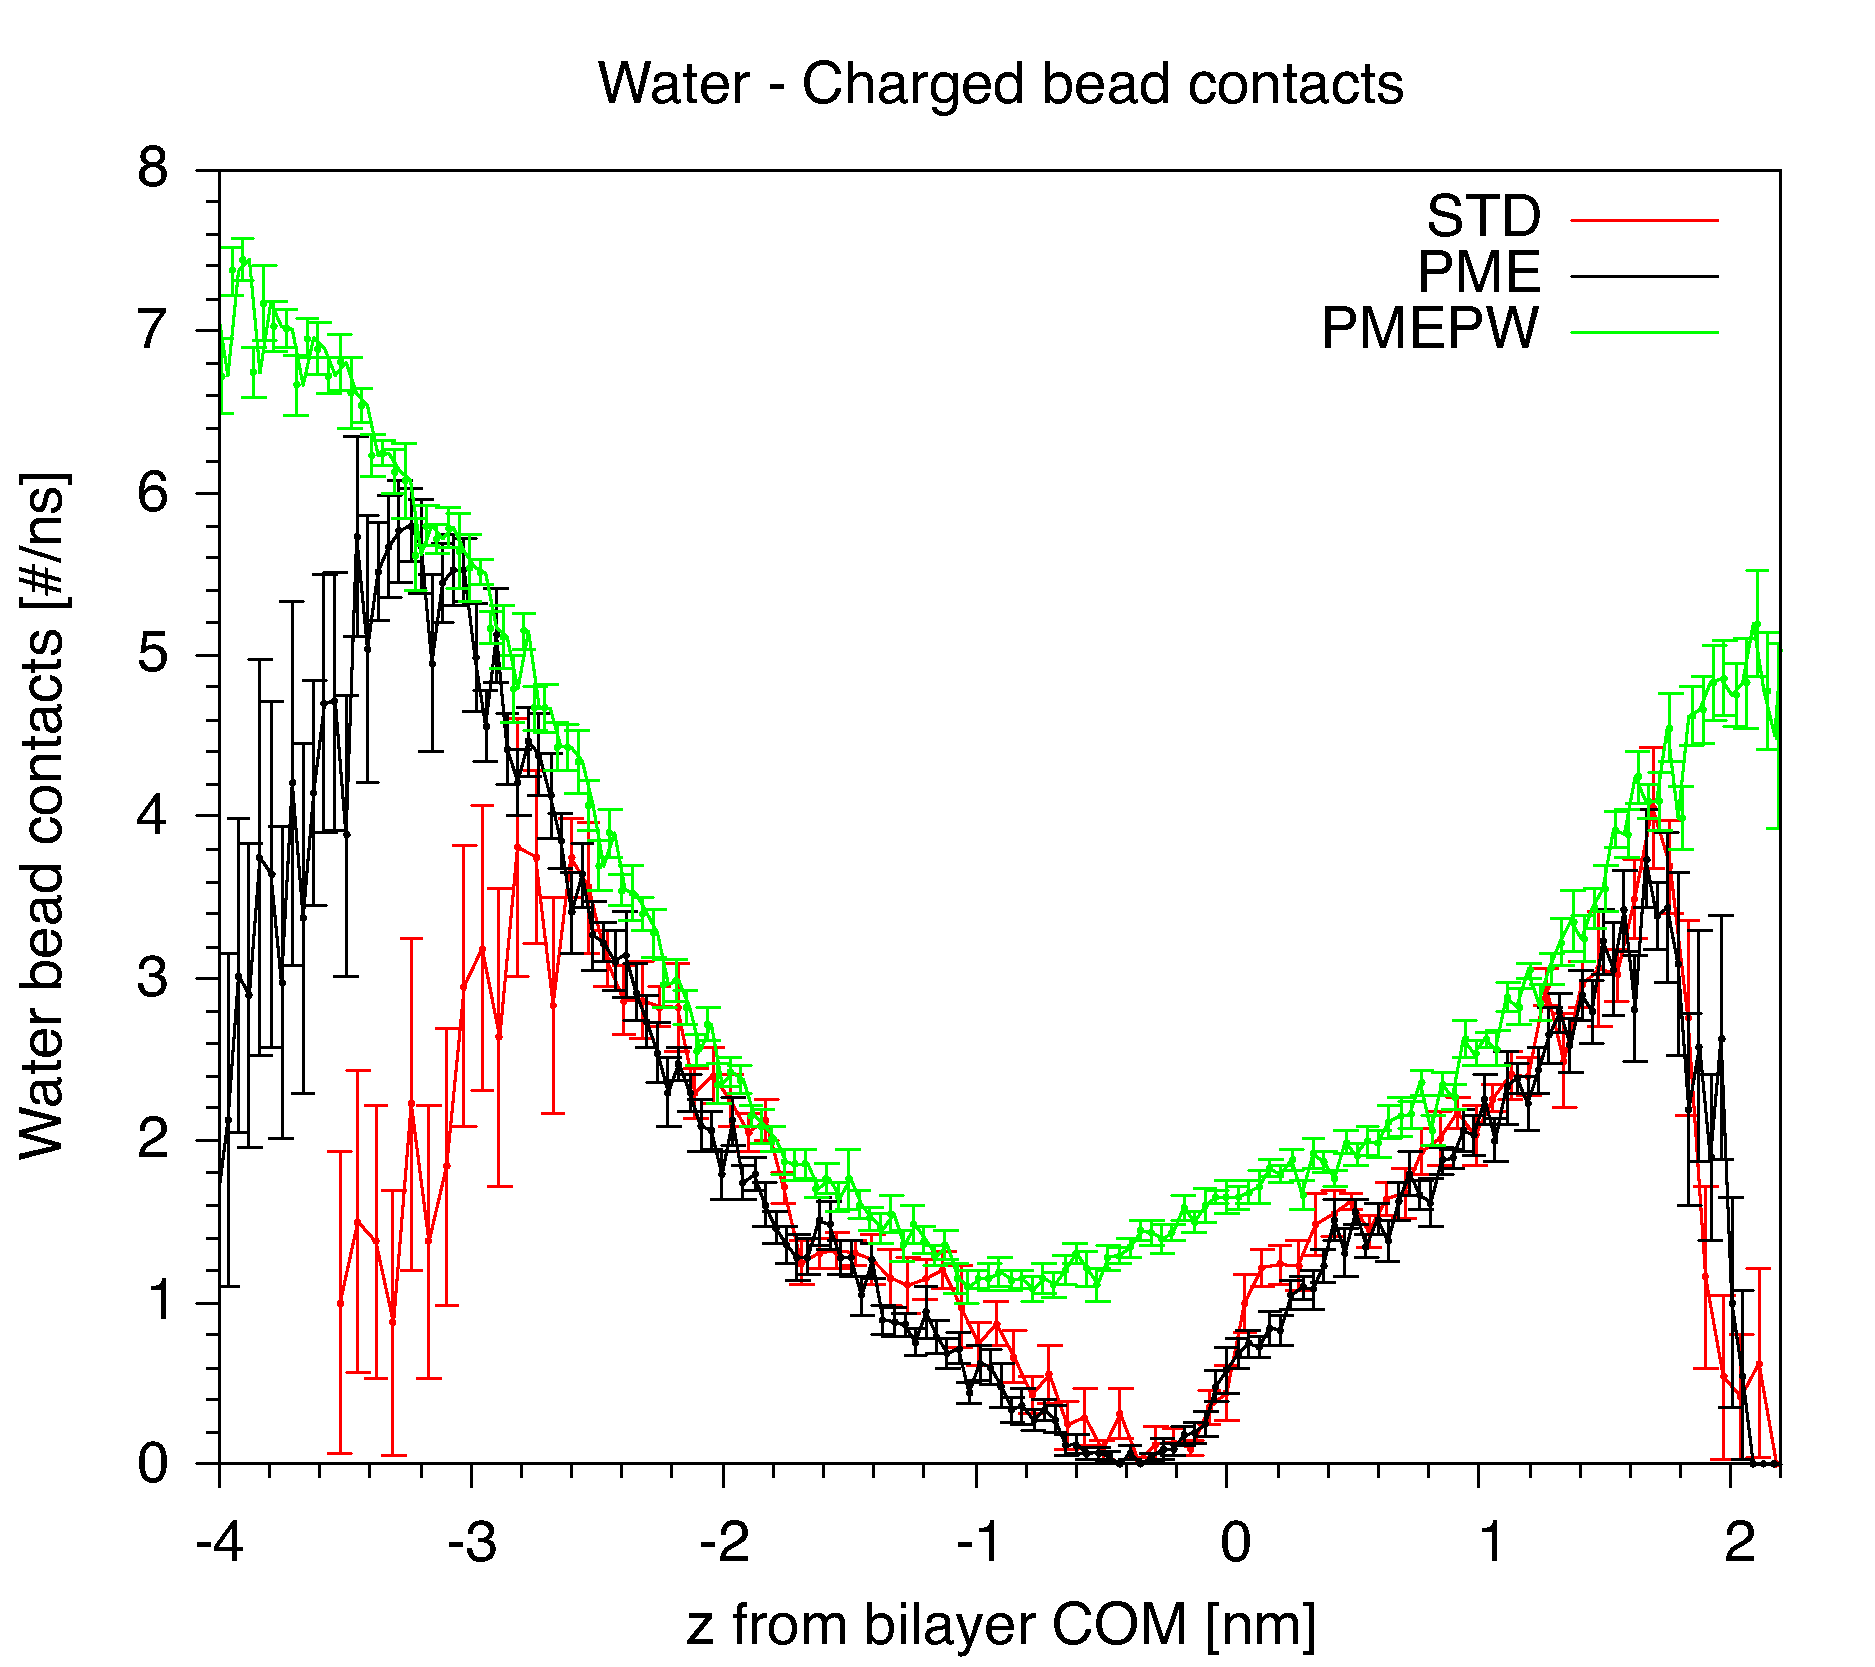
\includegraphics[width=0.5\textwidth]{./img/results/WPatchedComparison}
	}%
	\subfloat[striped – random comparison]{
		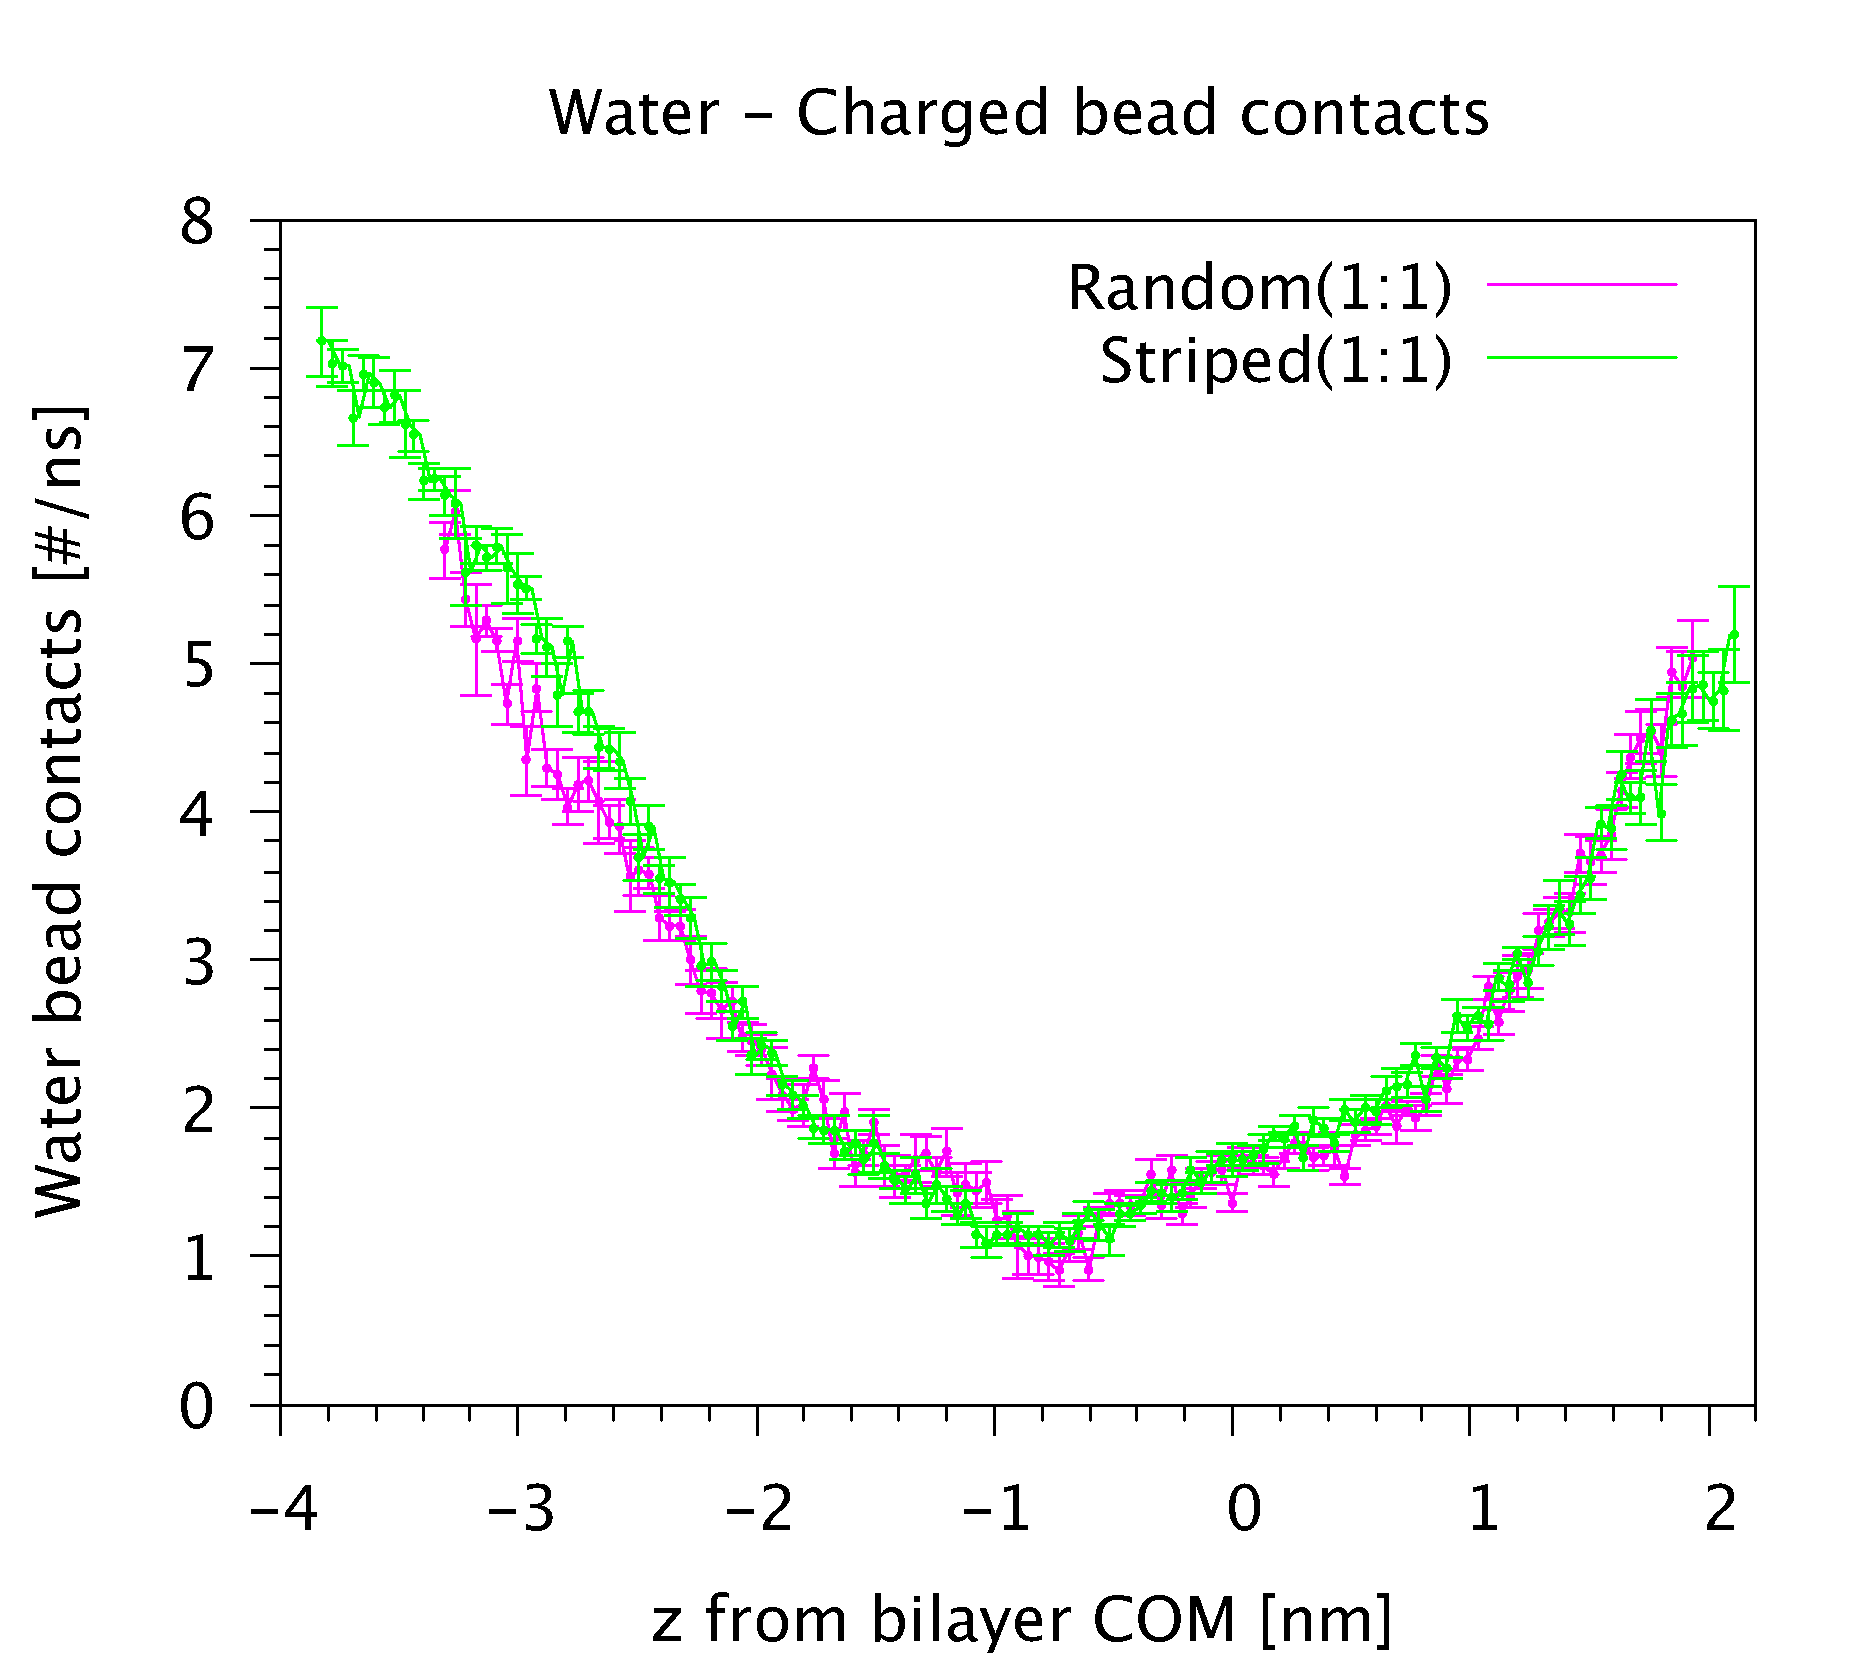
\includegraphics[width=0.5\textwidth]{./img/results/WRPComparison}
	}%
	\caption{Number of contacts per ns between water beads and the charged bead in function of the position of the charged bead. (a) For the striped \acs{NP} in comparison with different models. (b) In comparison between the striped and the random \acs{NP}s.}
	\label{fig:WContact}
\end{figure}
%\restoregeometry

As we can see from figure~(\ref{fig:WContact}a) for the standard \martini model and for the model with \ac{PME} alone we observe that the number of water contacts drop to zero in the core of the hydrophobic region. The contrary is observed for the model with the \ac{PW}, in which there is at least one contact per ns even in the core of the bilayer. Indeed we have to remark also that the persistence of the charged bead in the hydrophobic region is no more than $2$ or $3$~ns. The same behavior with the \ac{PW} model is observed also for the random \ac{NP}, shown in figure~(\ref{fig:WContact}b). For a comparison with the atomistic model we remark that the number of contacts per ns shown in the plots of figure~(\ref{fig:WContact}) have to be multiplied by four since one \martini water bead take into account to four real water molecules.

These results suggest that some \ac{PW} beads are dragged inside the hydrophobic region during the forward process, but also that some \ac{PW} beads, in the opposite leaflet, can help the anchoring process forming a water finger. The same behavior can apply to the backward process too.
 
% \begin{figure}[ht]
% 	\center
% 	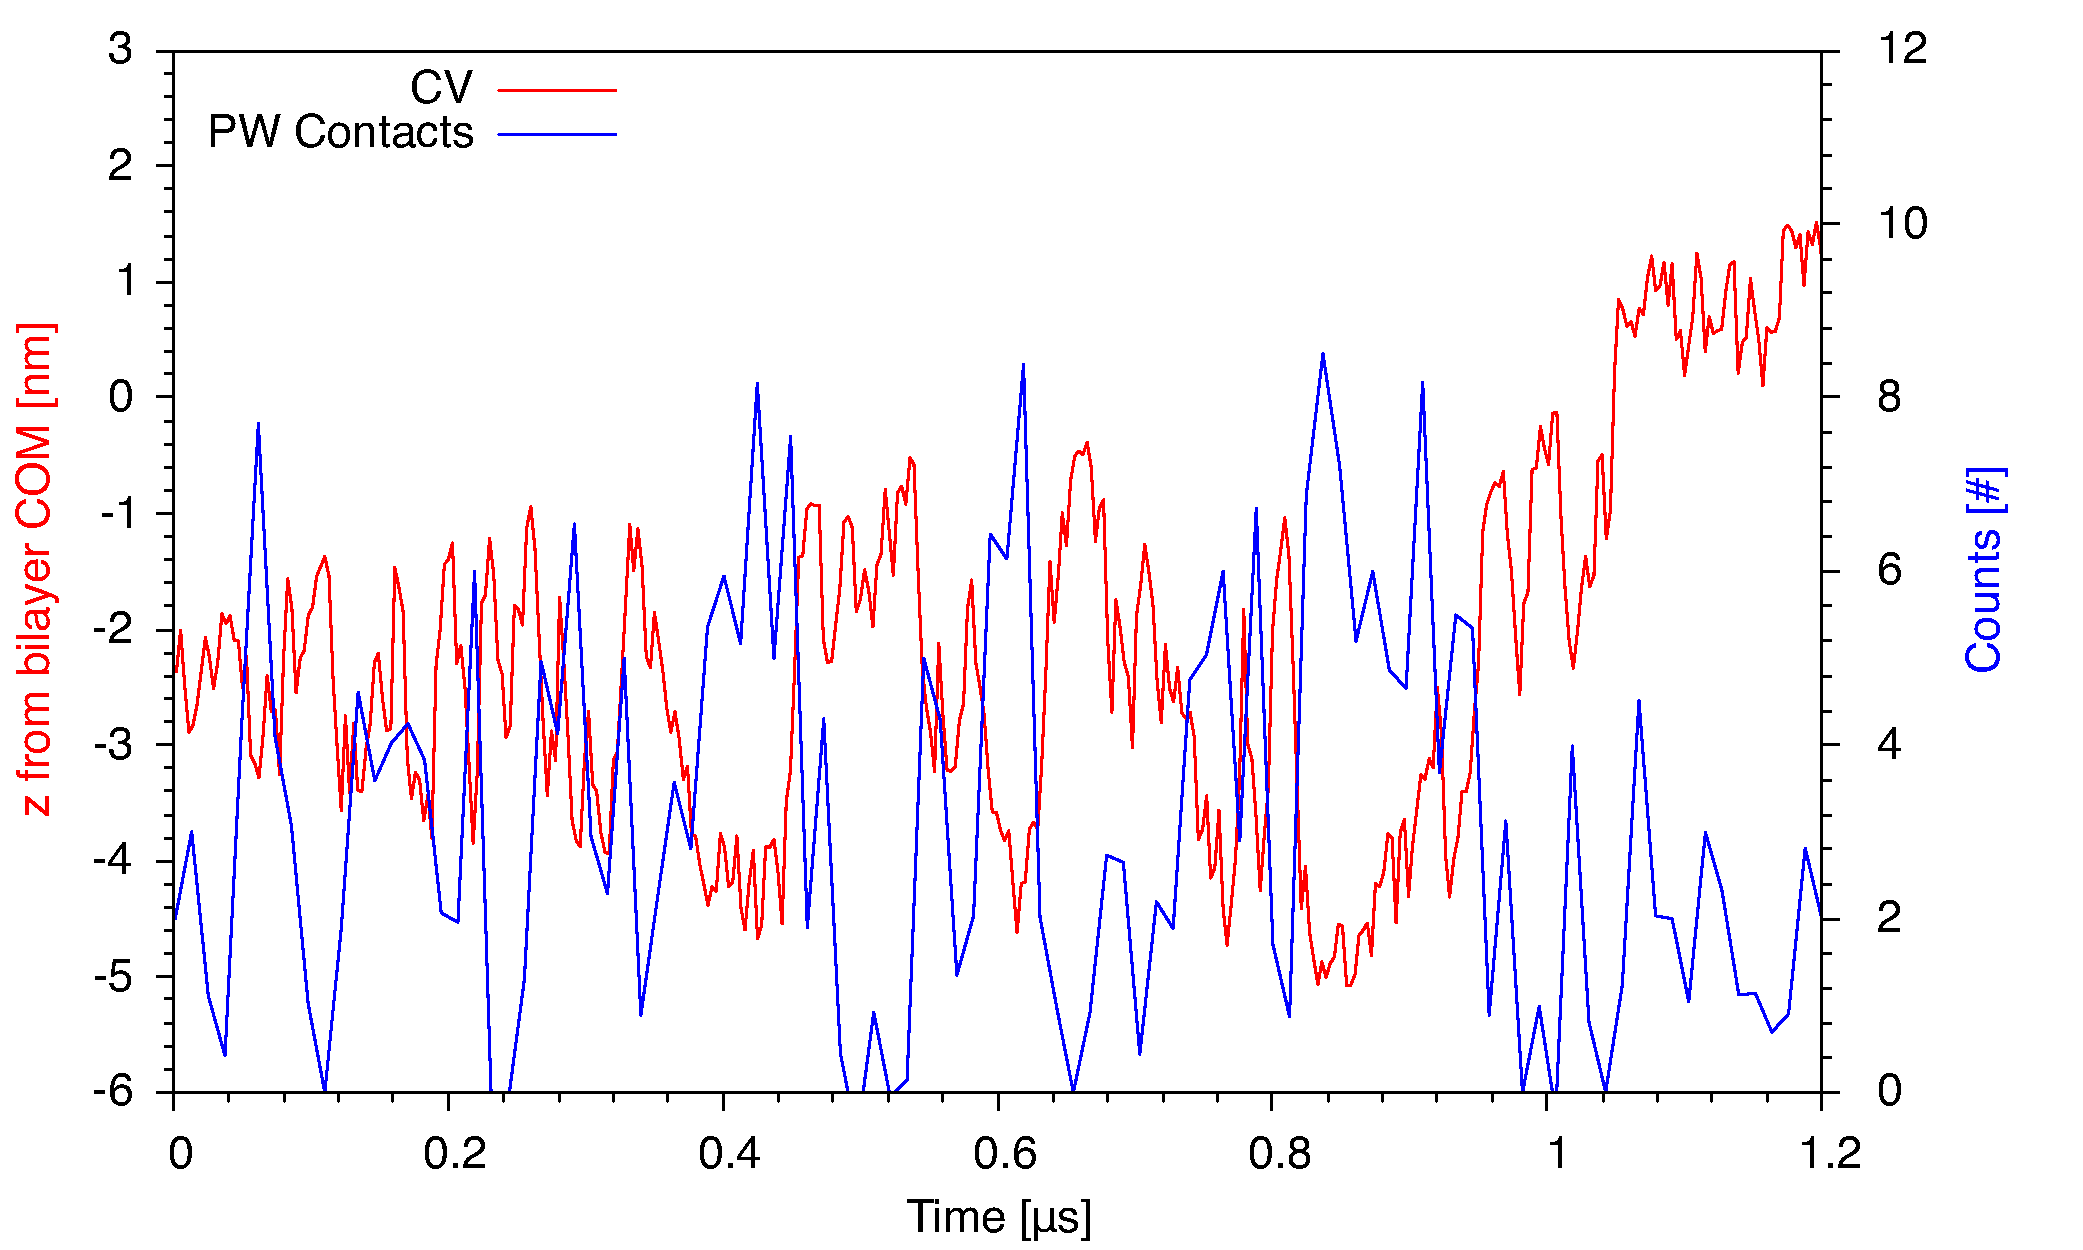
\includegraphics[width=0.9\textwidth]{./img/results/wCorrelation}
% 	\caption{Superposition of the \acs{CV} (red) and the number of contacts between the \acs{PW} beads and the charged bead (blue) in function of the time for a striped metadyamcis run. $z>0$ corresponds to the anchored state. It can be noted a clear anti--correlation between the distance of the charged bead from the bilayer \acs{COM} and the number of the \acs{PW} contacts: they decrease when the charged bead is approaching the hydrophobic region.}
% \end{figure}

\section{Lipid heads dragging}
%Trascinamento delle teste dei lipidi nelle varie salse
The same dragging effect of the water beads during the forward process, is also noticed for the coline group (NC$3$ bead) of the entrance leaflet. In order to have a qualitatively idea of the phenomena, for all the NC$3$ beads in the entrance leaflet, we have calculated the closer to the bilayer \ac{COM} in function of the time. Then, plotting its $z$ distance from the bilayer \ac{COM}, together with the $z$ distance of the charged bead, in function of the time I get the plot shown in figure~(\ref{fig:NC3Correlation}). We can see an evidently correlation: when the ligand tends to approach the opposite leaflet the smallest distance of the NC$3$ beads drop to zero at the same time. This suggest that some NC$3$ bead is strongly bound to the charged bead and it tend to drag the head lipid inside the hydrophobic region. Since the flip-flopping energy for a \ac{POPC} lipid is too high, when the charged bead is too far from the entrance leaflet the NC$3$ bead detaches and go back to the entrance leaflet. 
\begin{figure}[ht]
	\center
	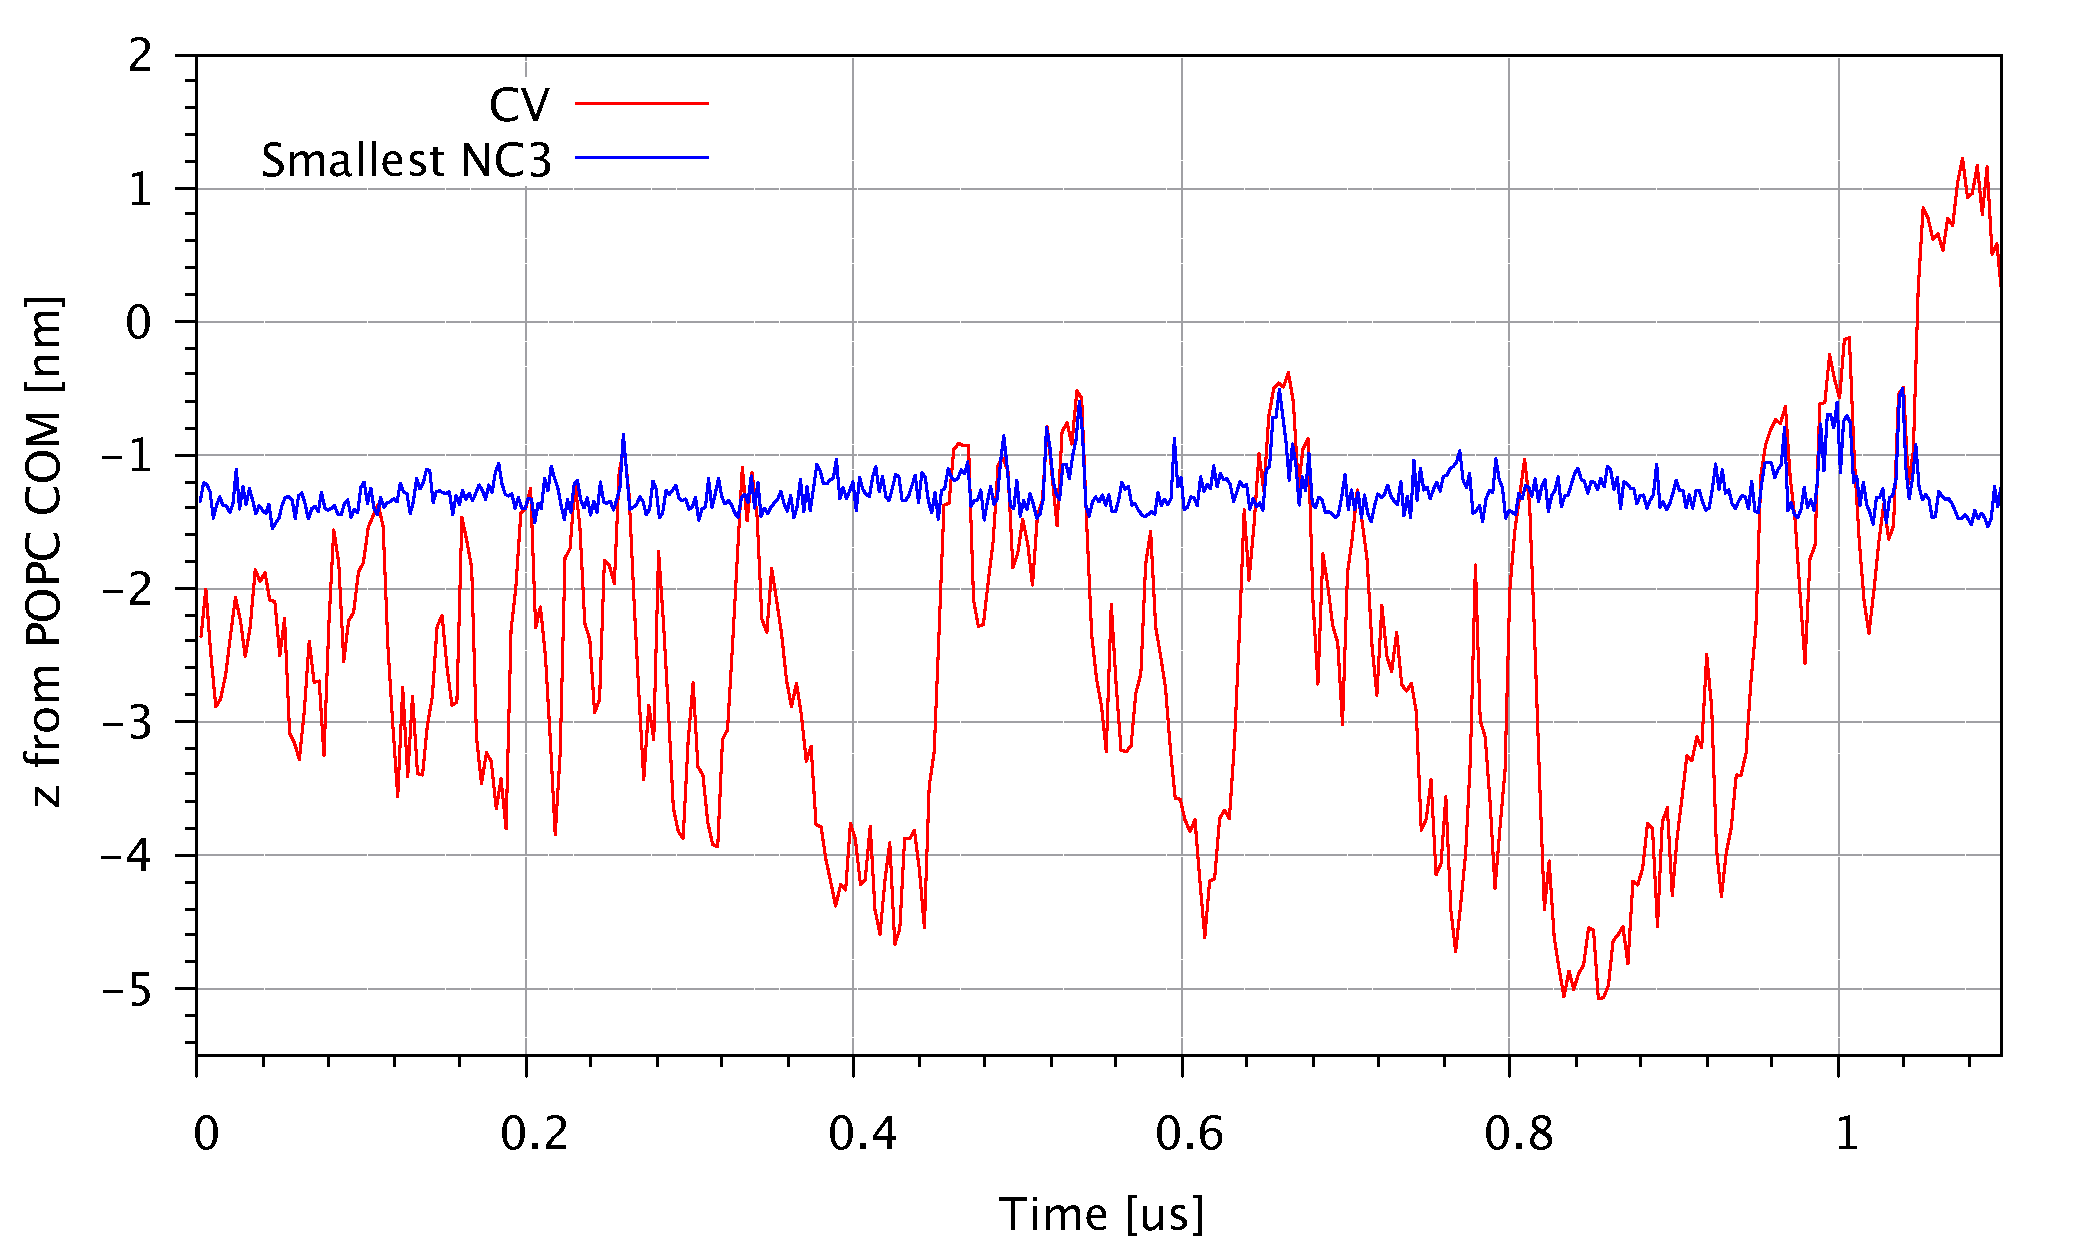
\includegraphics[width=0.9\textwidth]{./img/results/NC3Correlation}
	\caption{Superposition of the \acs{CV} (red) and the smallest $z$ distance from bilayer \acs{COM} of the NC$3$ beads of the entrance leaflet (blue) in function of the time for a striped metadynamics run. $z>0.5$ corresponds to the anchored state. It can be noted a clear correlation between them: the NC$3$ bead closer to the bilayer \acs{COM} follow the charged bead approaching the opposite leaflet.}
	\label{fig:NC3Correlation}
\end{figure}

% 	minDistPatched			minDistRandom11
\begin{figure}[h!p]
	\center
	\subfloat[striped NP]{
		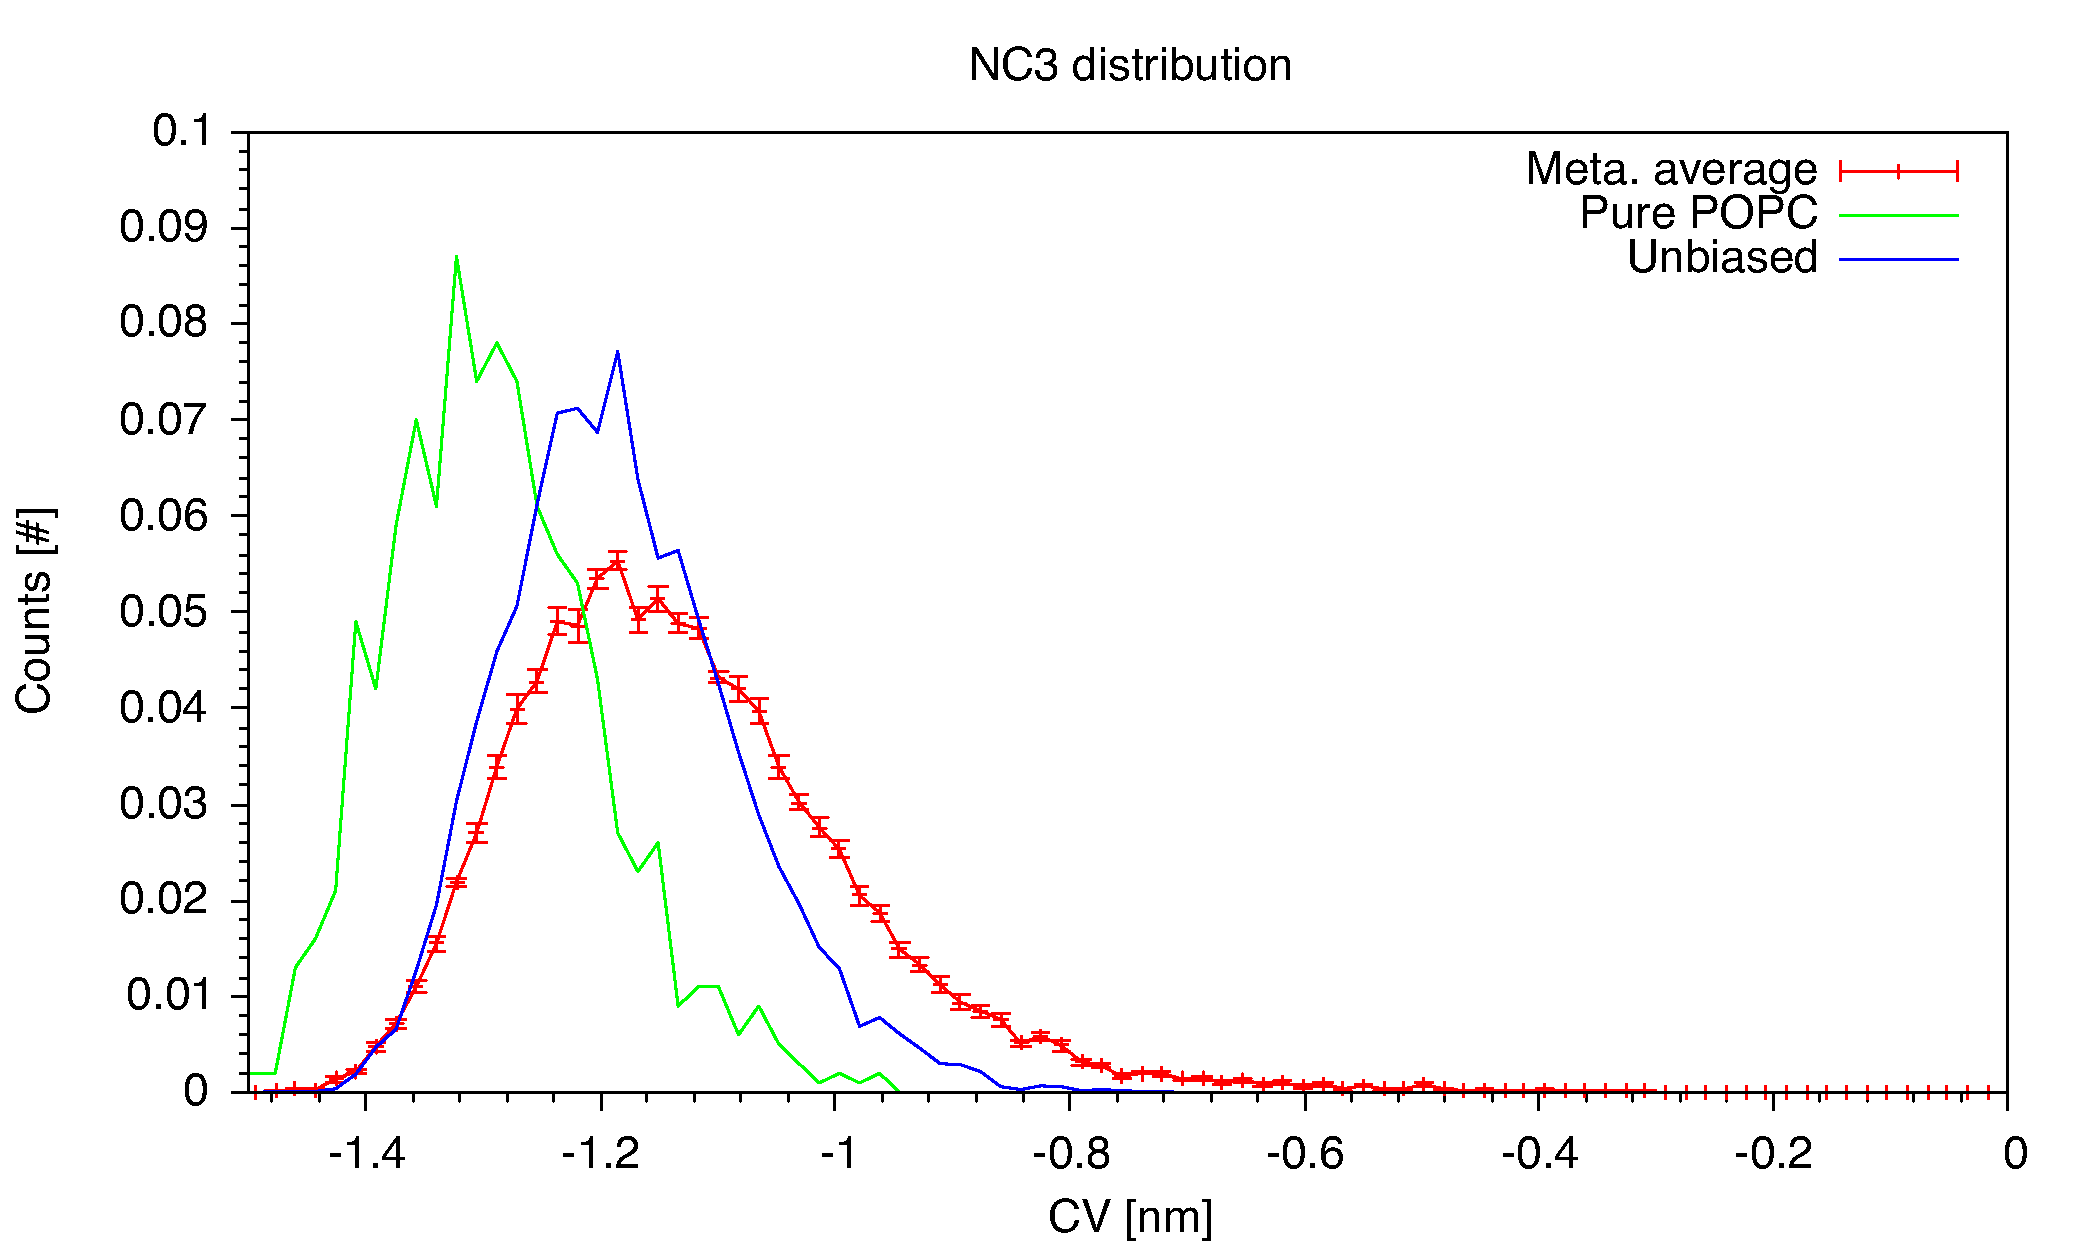
\includegraphics[width=\textwidth]{./img/results/minDistPatched}
	}\\%
	\subfloat[random NP]{
		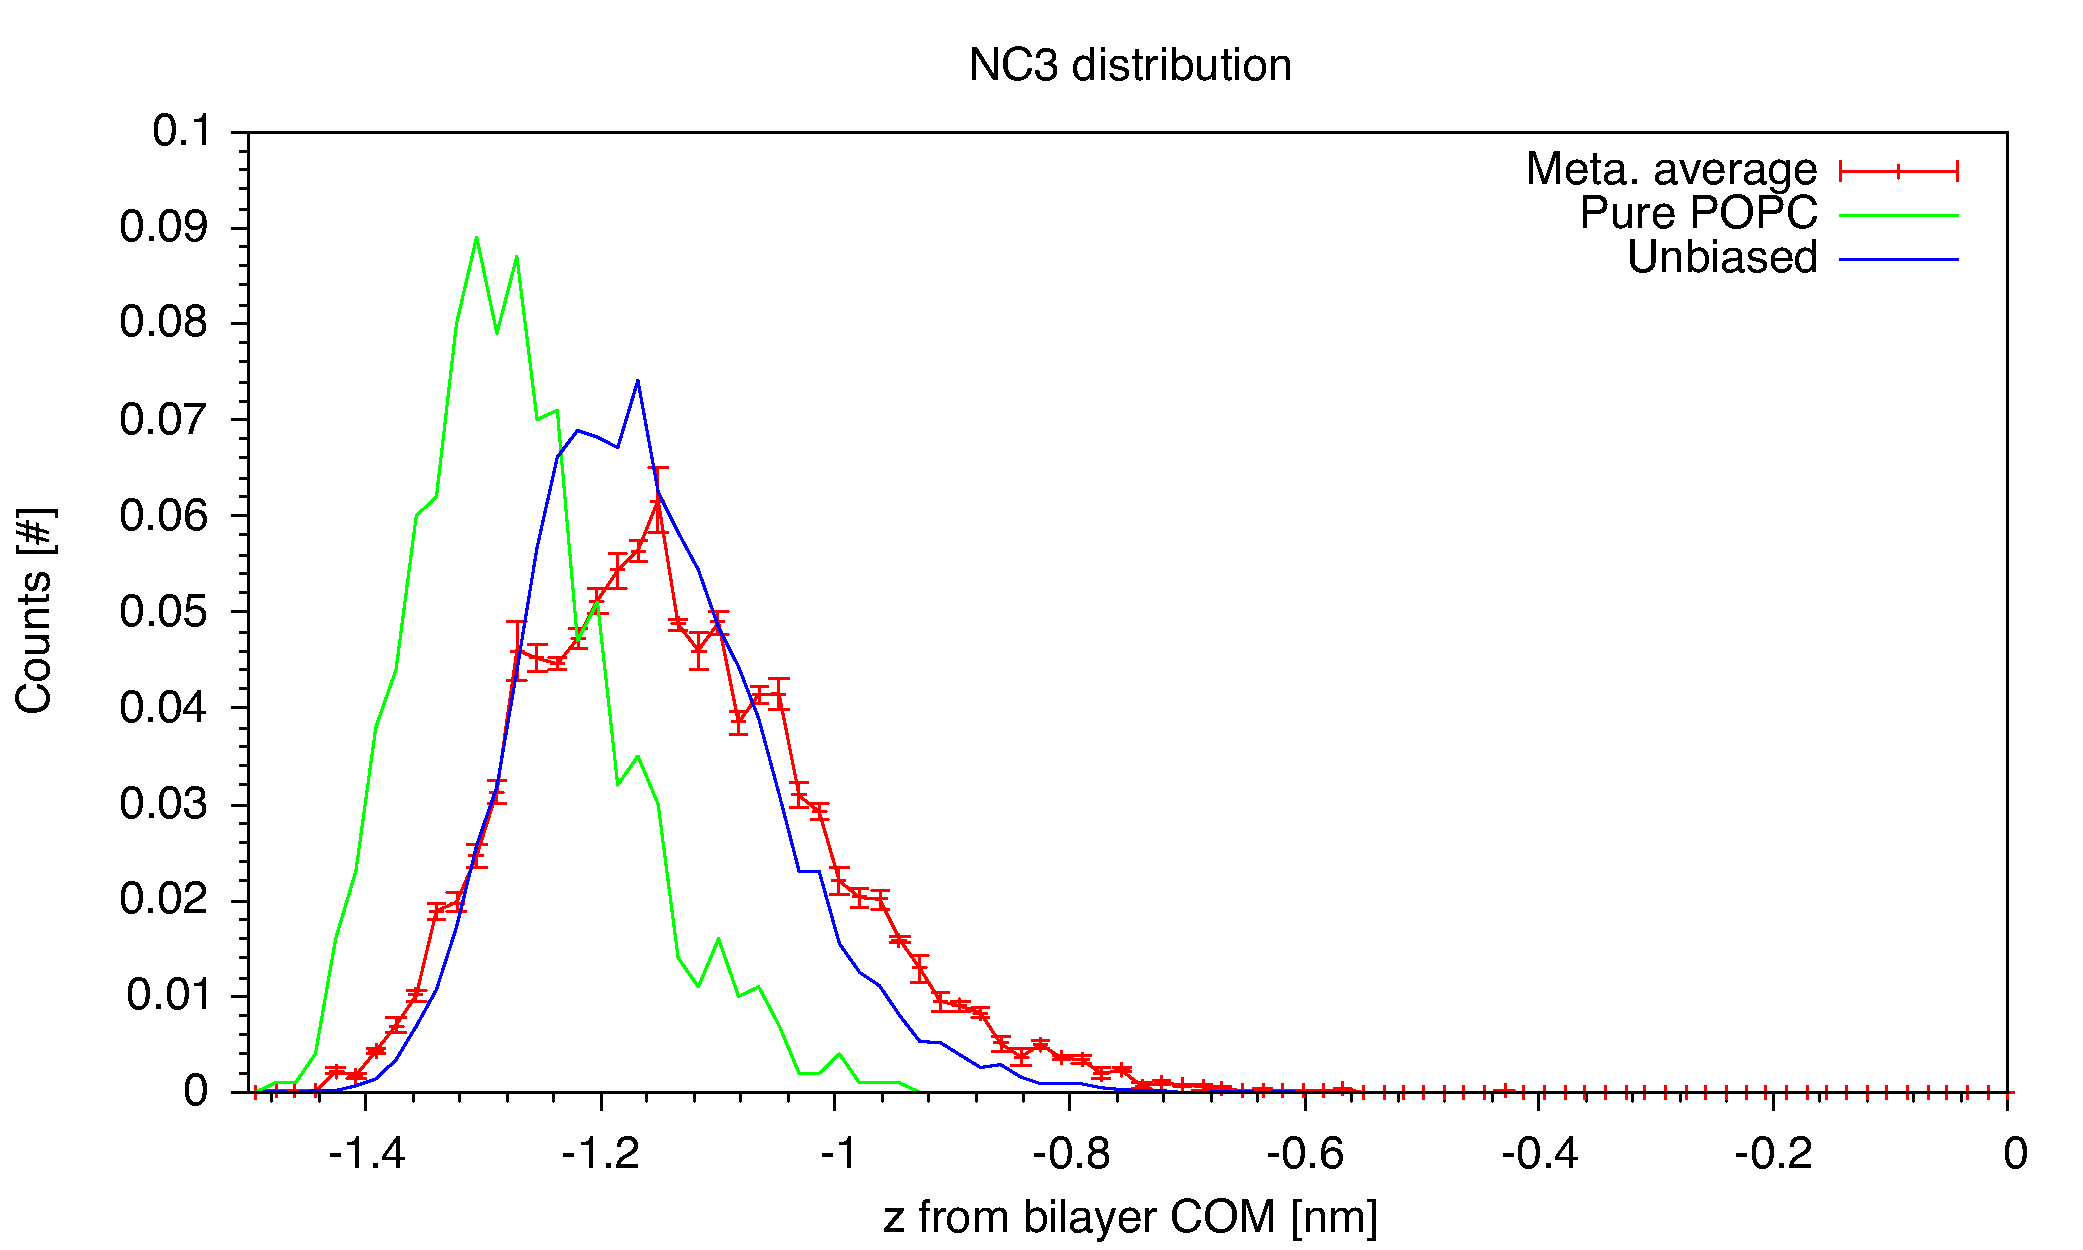
\includegraphics[width=\textwidth]{./img/results/minDistRandom11}
	}%
	\caption{Average distribution of the coline groups (NC3 beads) in the entrance leaflet closer to the bilayer \acs{COM} in function of the position of the charged bead in comparison with an average over ten metadynamics runs, the unbiased run and a pure \acs{POPC} run for: (a) the striped \acs{NP} and (b) the random \acs{NP}.}
	\label{fig:NC3minDist}
\end{figure}

In order to better investigate such process and for a comparison with different models and \ac{NP} configurations to be made, in figure~(\ref{fig:NC3minDist}) is shown an histogram of the distribution of the NC$3$ beads in the entrance leaflet closer to the bilayer \ac{COM} in function of the $z$ distance from the bilayer \ac{COM}, in a comparison with a pure \ac{POPC} bilayer, an unbiased run and an average over all the metadynamics runs for the striped \ac{NP}, figure~(\ref{fig:NC3minDist}a) and the random one, figure~(\ref{fig:NC3minDist}b). All the data are from runs with both \ac{PME} and \ac{PW}. The bin width is $0.02$~nm for all curves and each histogram is normalized to the total number of entries. The error bar for the metadynamics runs is calculated as the standard error of the mean value.

%	NC3PatchedComparison	NC3RPComparison
%\newgeometry{left=2.5cm,right=2.5cm}
\begin{figure}
	\center
	\subfloat[striped – model comparison]{
		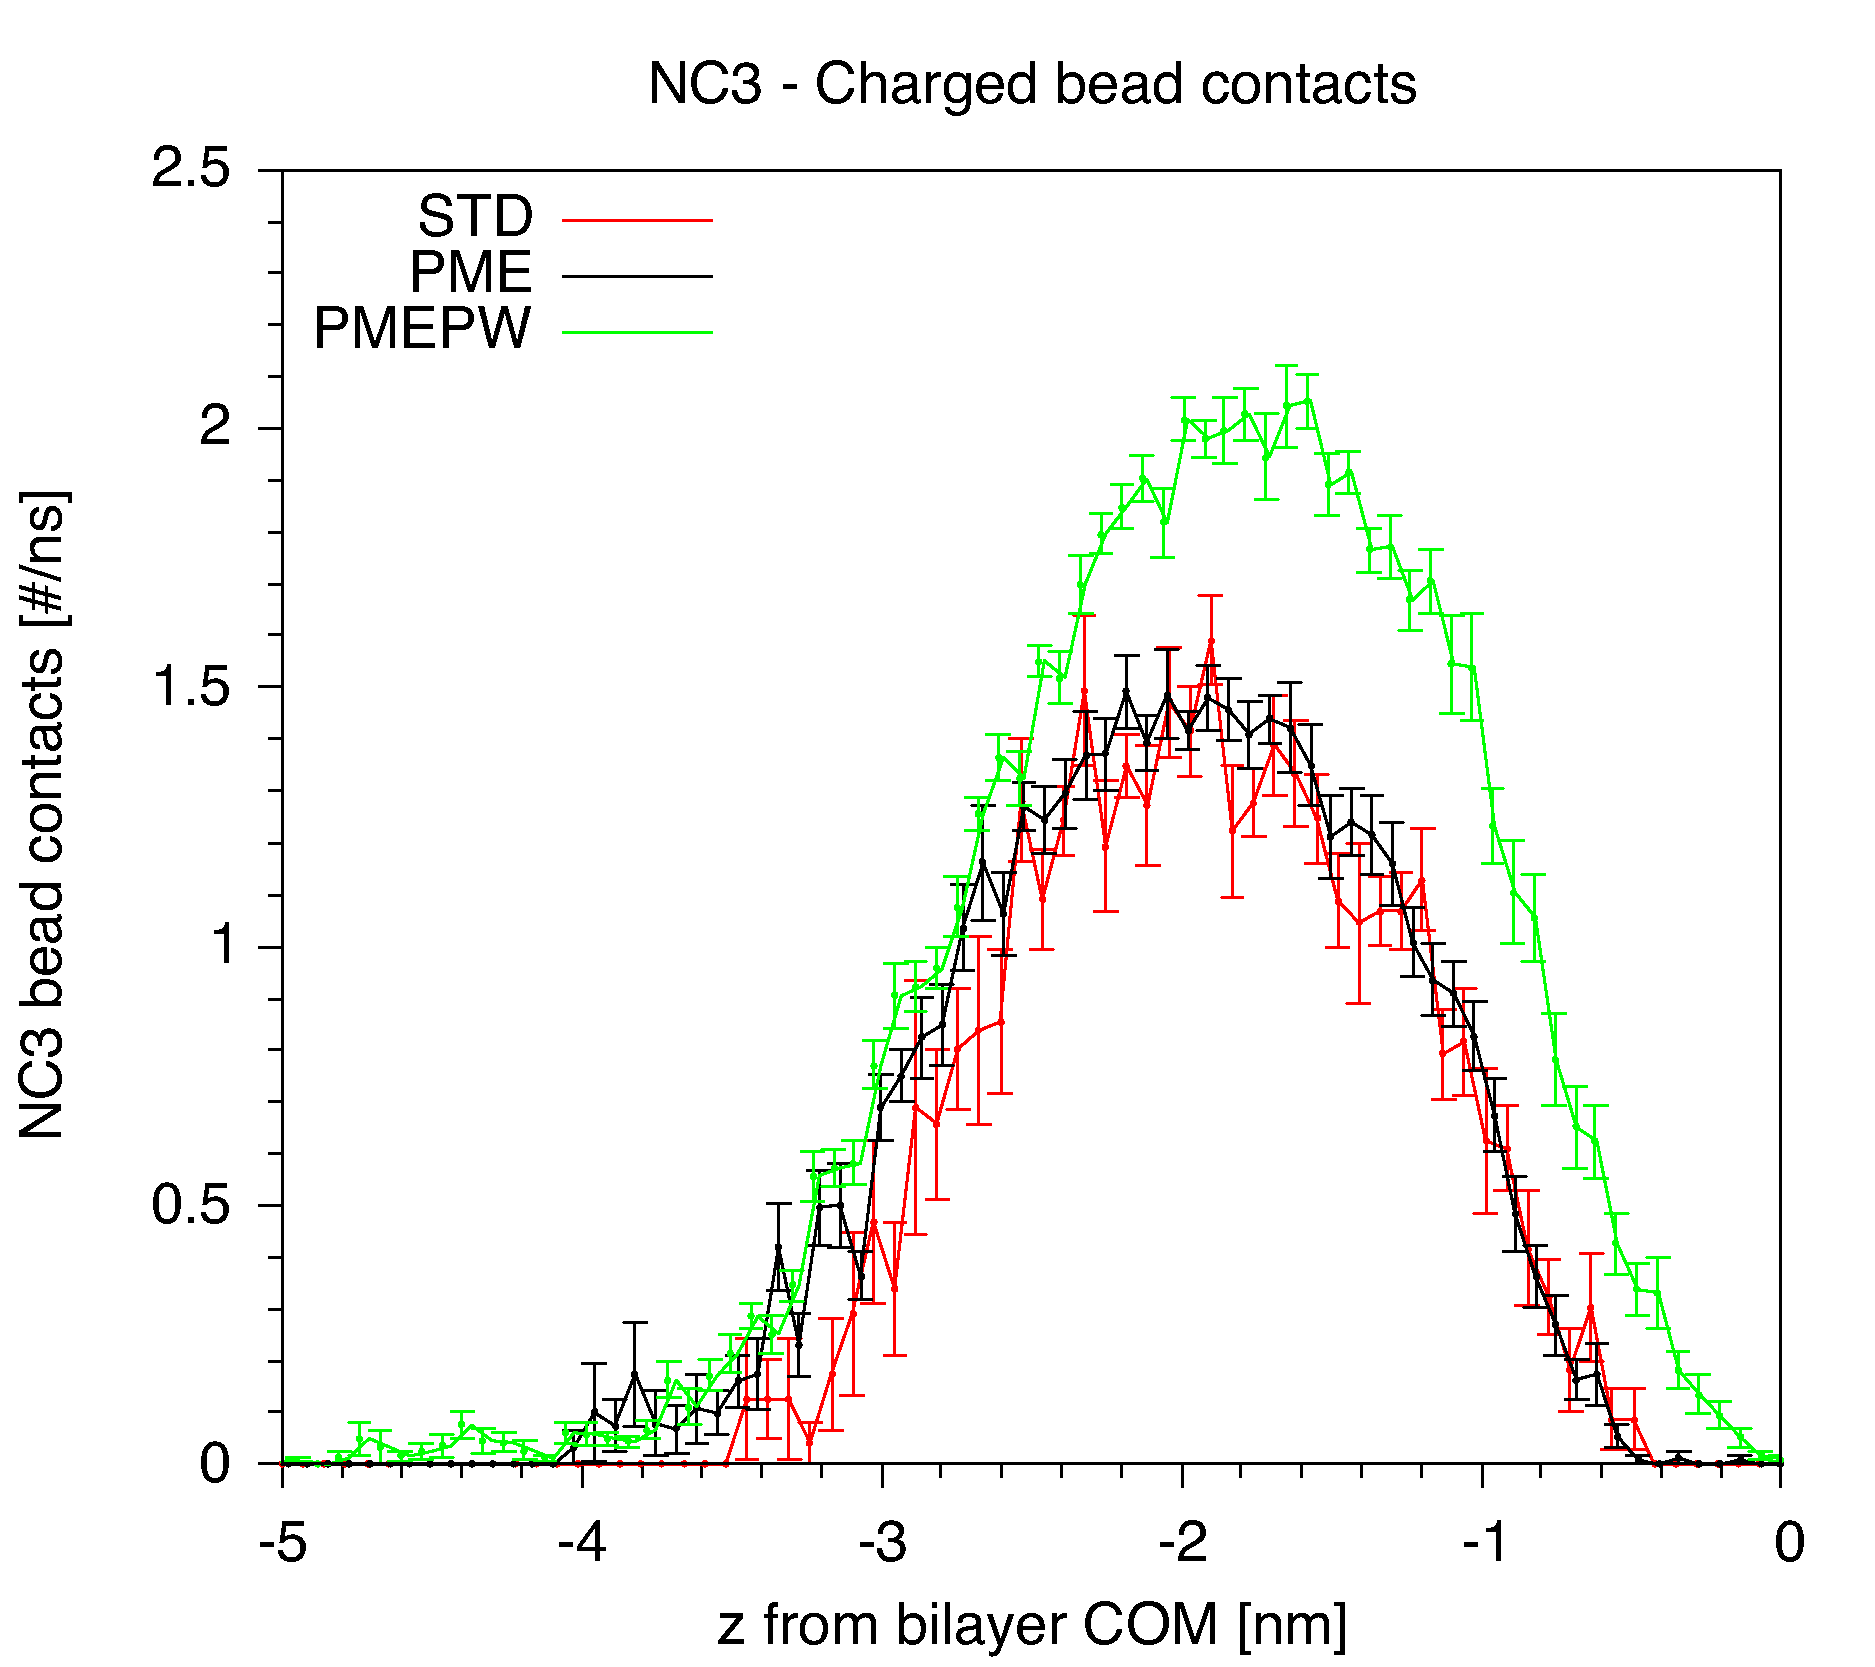
\includegraphics[width=0.5\textwidth]{./img/results/NC3PatchedComparison}
	}%
	\subfloat[striped – random comparison]{
		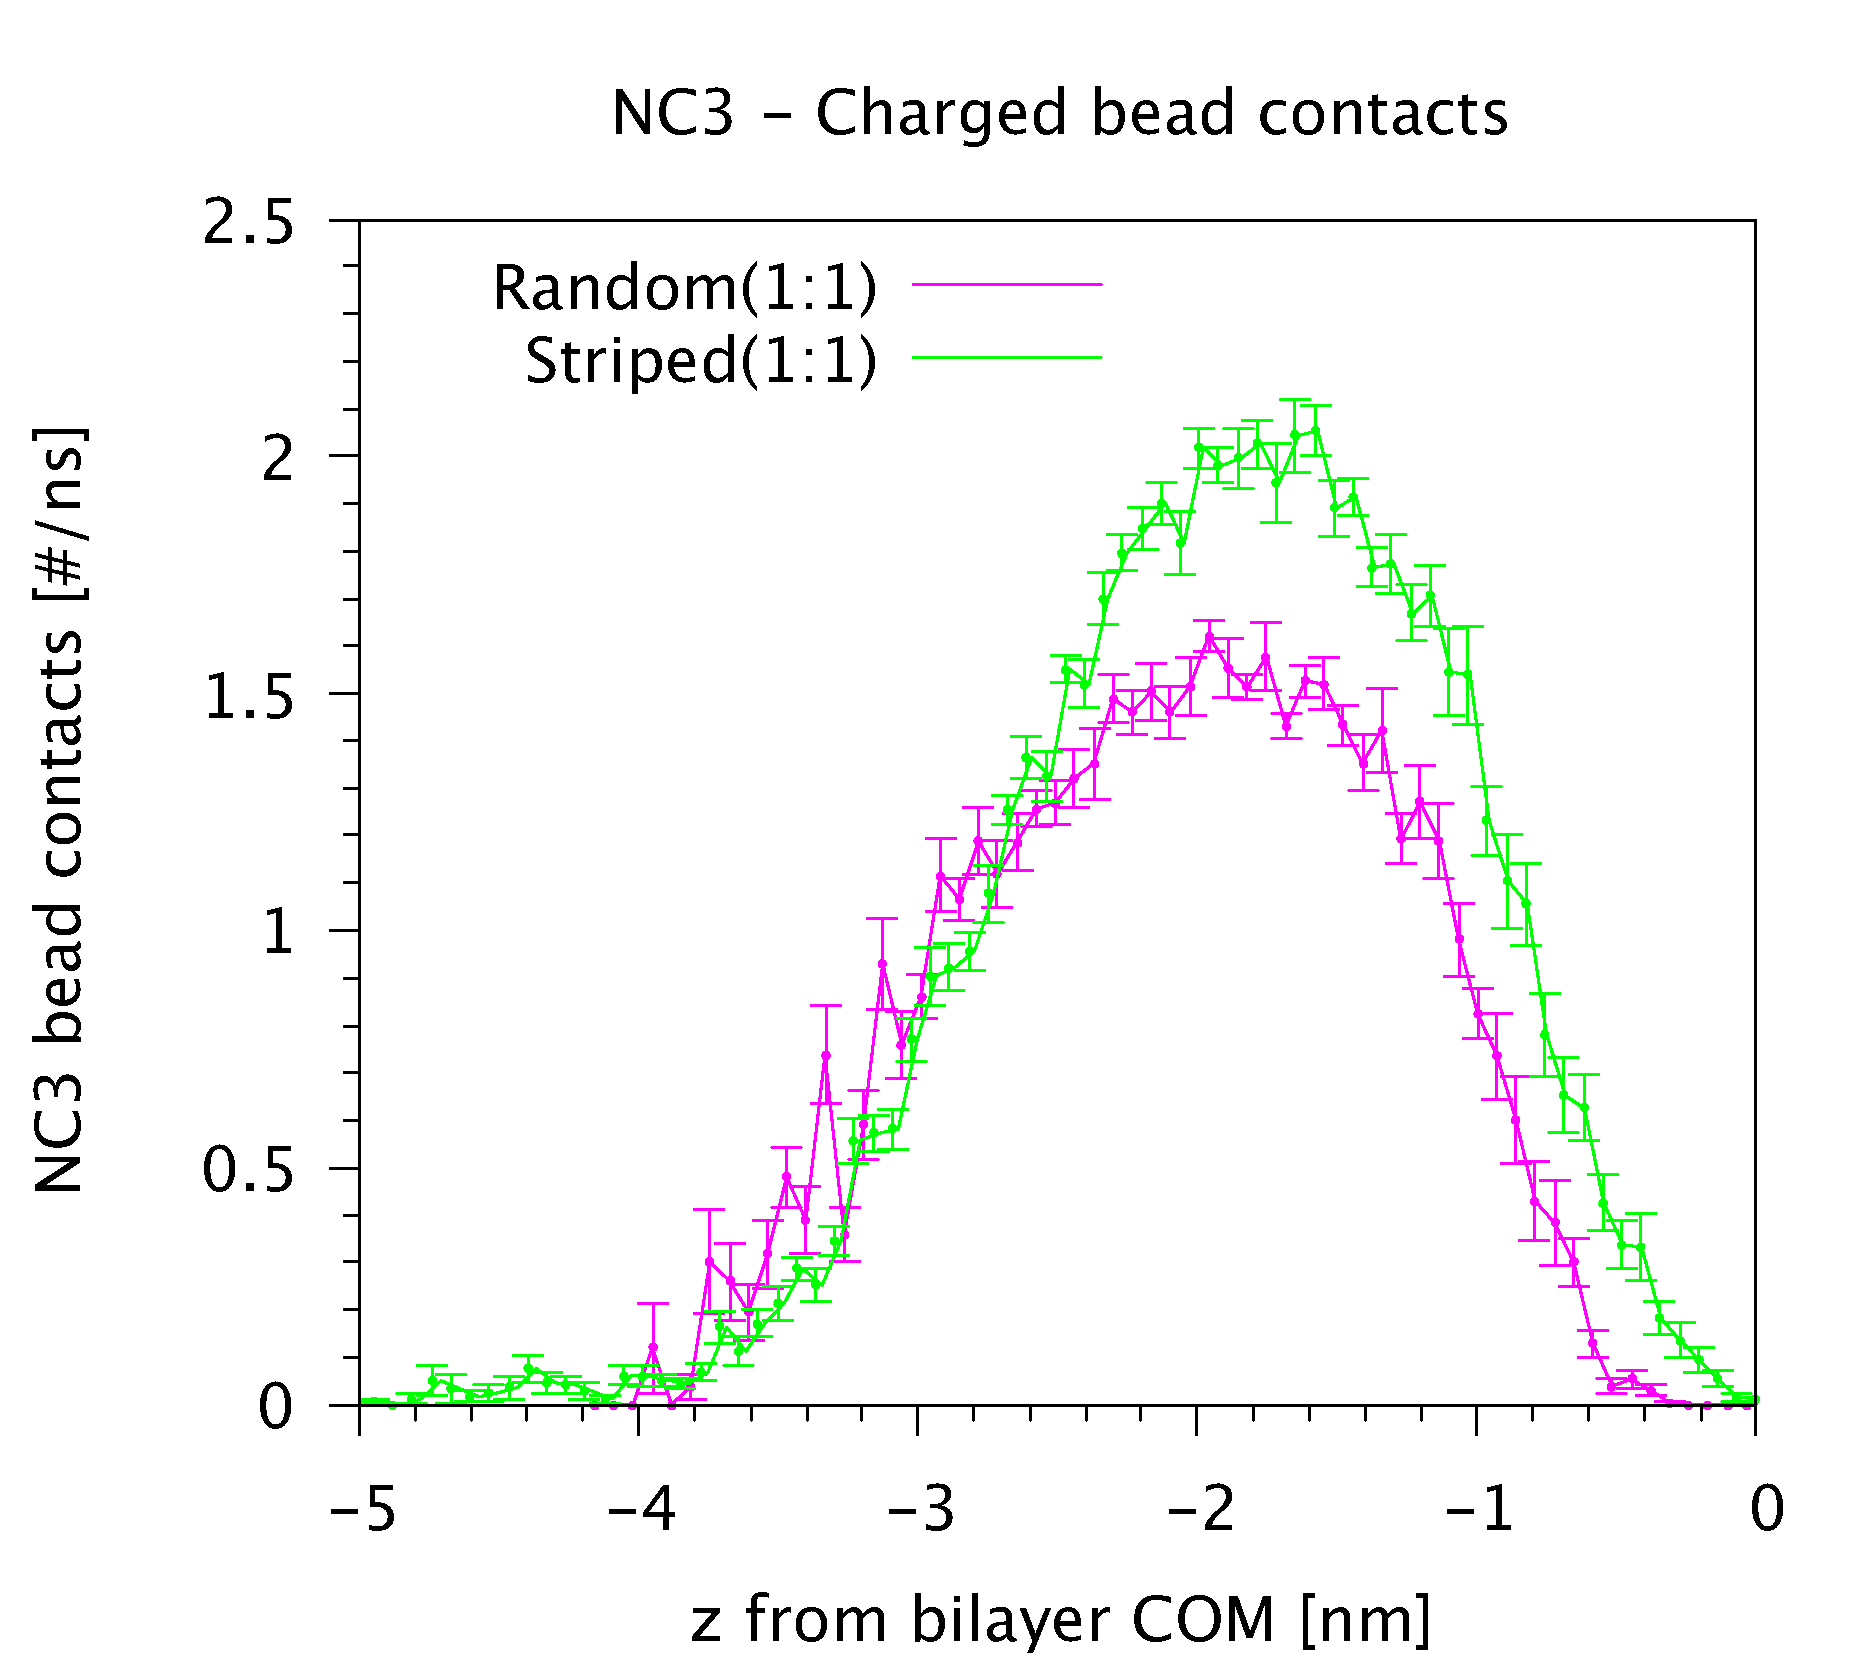
\includegraphics[width=0.5\textwidth]{./img/results/NC3RPComparison}
	}%
	\caption{Number of contacts per ns between coline group (NC3 bead) and the charged bead in function of the position of the charged bead in the hydrophobic state. (a) For the striped \acs{NP} in comparison with different models. (b) In comparison between the striped and the random \acs{NP}s. Data from my runs with \acs{PME} and \acs{PW}.}
	\label{fig:NC3Contact}
\end{figure}
%\restoregeometry

Moreover, the same analysis for the water contacts as described in~\ref{sec:WDragging}, is made even for the contacts of the NC$3$ beads in the entrance leaflet within $0.6$~nm from the charged bead. The bin width is $0.08$~nm. The analysis results are shown in figure~(\ref{fig:NC3Contact}. In particular, in figure~(\ref{fig:NC3Contact}a) is shown a comparison with different \ac{CG} \martini models: the standard, with \ac{PME} alone and with both \ac{PME} and \ac{PW}. Instead, in figure~(\ref{fig:NC3Contact}b) is shown a comparison between the striped and the random \acp{NP} with \ac{PME} and \ac{PW}. We see that with the \ac{PW} model the contacts per ns are still appreciable even near the core of the membrane. This and the previous results confirm the dragging effect of the head lipids of the entrance leaflet by the charged bead during the forward process. In the random--striped comparison we see that this effect is less noticeable for the random \ac{NP} and the number of contacts is globally lower respect to the striped one. This can be consistence with the fact that the average $z$ distance of the \ac{NP} \ac{COM} from the bilayer \ac{COM} is less for the striped than that for the random one, as shown in table~(\ref{tab:NPMembProperties}). 


\section{Effects of metadynamics}
%Quanto la metadinamica sia distrittiva: comparazione tra rum unbiased e biased
We have used the metadynamics to estimate the energy barriers of the forward and the backward process. In order to qualitatively understand if the metadynamics alters the simulation we can compare the previous results with the one obtained with the unbiased runs. In figure~(\ref{fig:NC3minDistUn}) is shown the NC$3$ distribution closer to bilayer \ac{COM} in function of the $z$ distance form the bilayer \ac{COM} in which for the metadynamics runs only the portion of the trajectory in which the \ac{NP} is in the hydrophobic state is considered. Then in figure~(\ref{fig:contactsUn}) is shown the number of contacts for water and the NC$3$ for the striped and the random \acp{NP} in a comparison between the metadynamics and the unbiased runs. These analyzes are made considering only the \ac{PME} plus \ac{PW} model. From figure~(\ref{fig:contactsUn}) we see that the number of contacts are almost equal in the hydrophobic state for all plots, suggesting that the metadynamics is non--destructive. Instead, for the NC$3$ distribution closer to the center of the bilayer we observe an appreciable count neat the hydrophobic core of the bilayer, even if only the hydrophobic state is considered. This suggest that the head lipids dragging is present due to the oscillation of the charged bead exploring a bigger area of the \ac{CV} phase space when the \ac{NP} is still in the hydrophobic state.
% 	minDistHydroPatched		minDistHydroRandom11
\begin{figure}[!bh]
	\center
	\subfloat[striped NP]{
		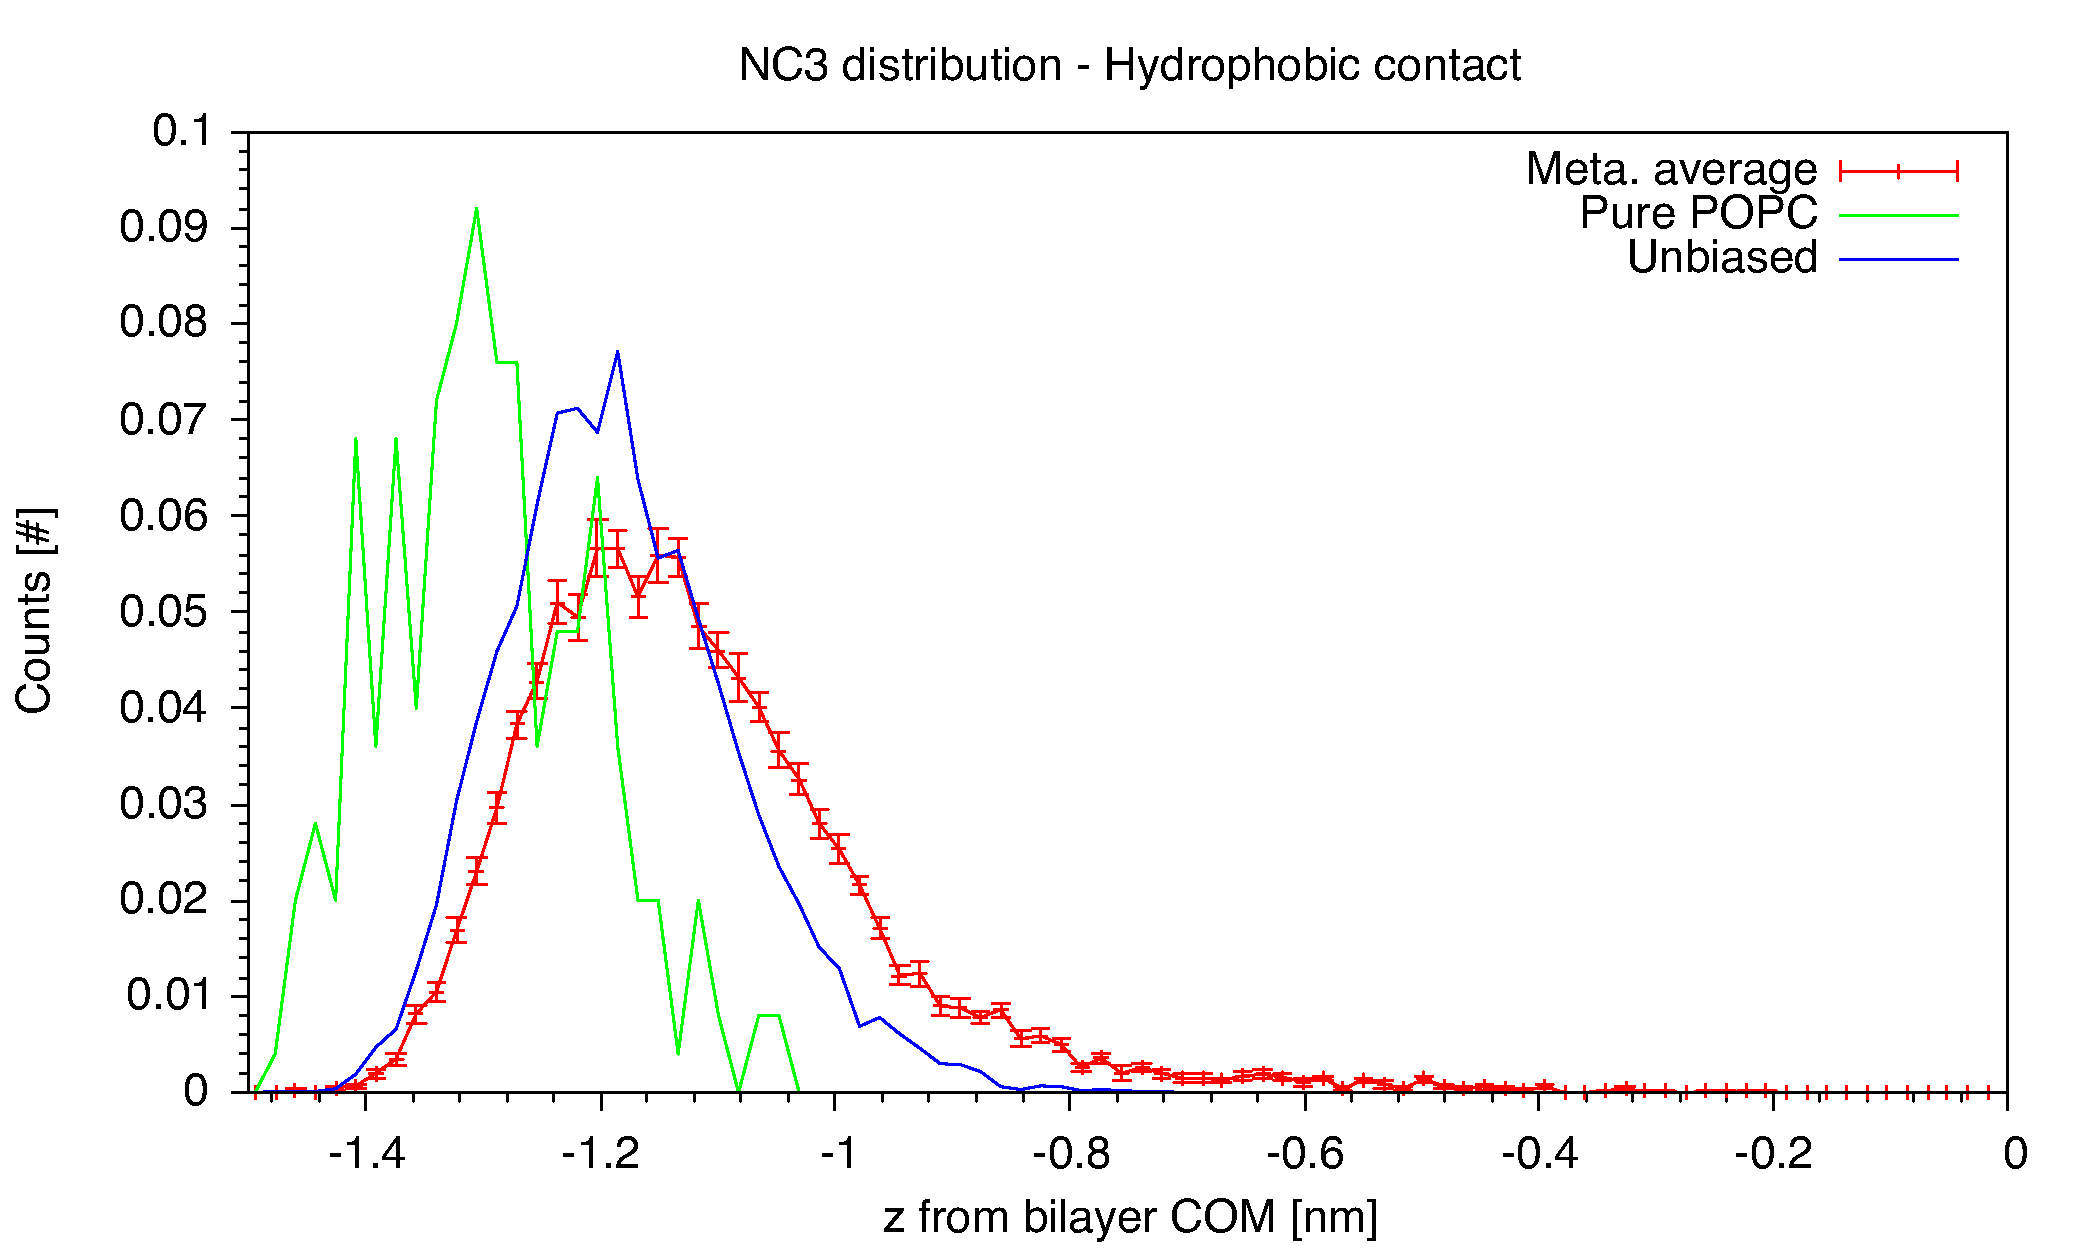
\includegraphics[width=0.95\textwidth]{./img/results/minDistHydroPatched}
	}\\%
	\subfloat[random NP]{
		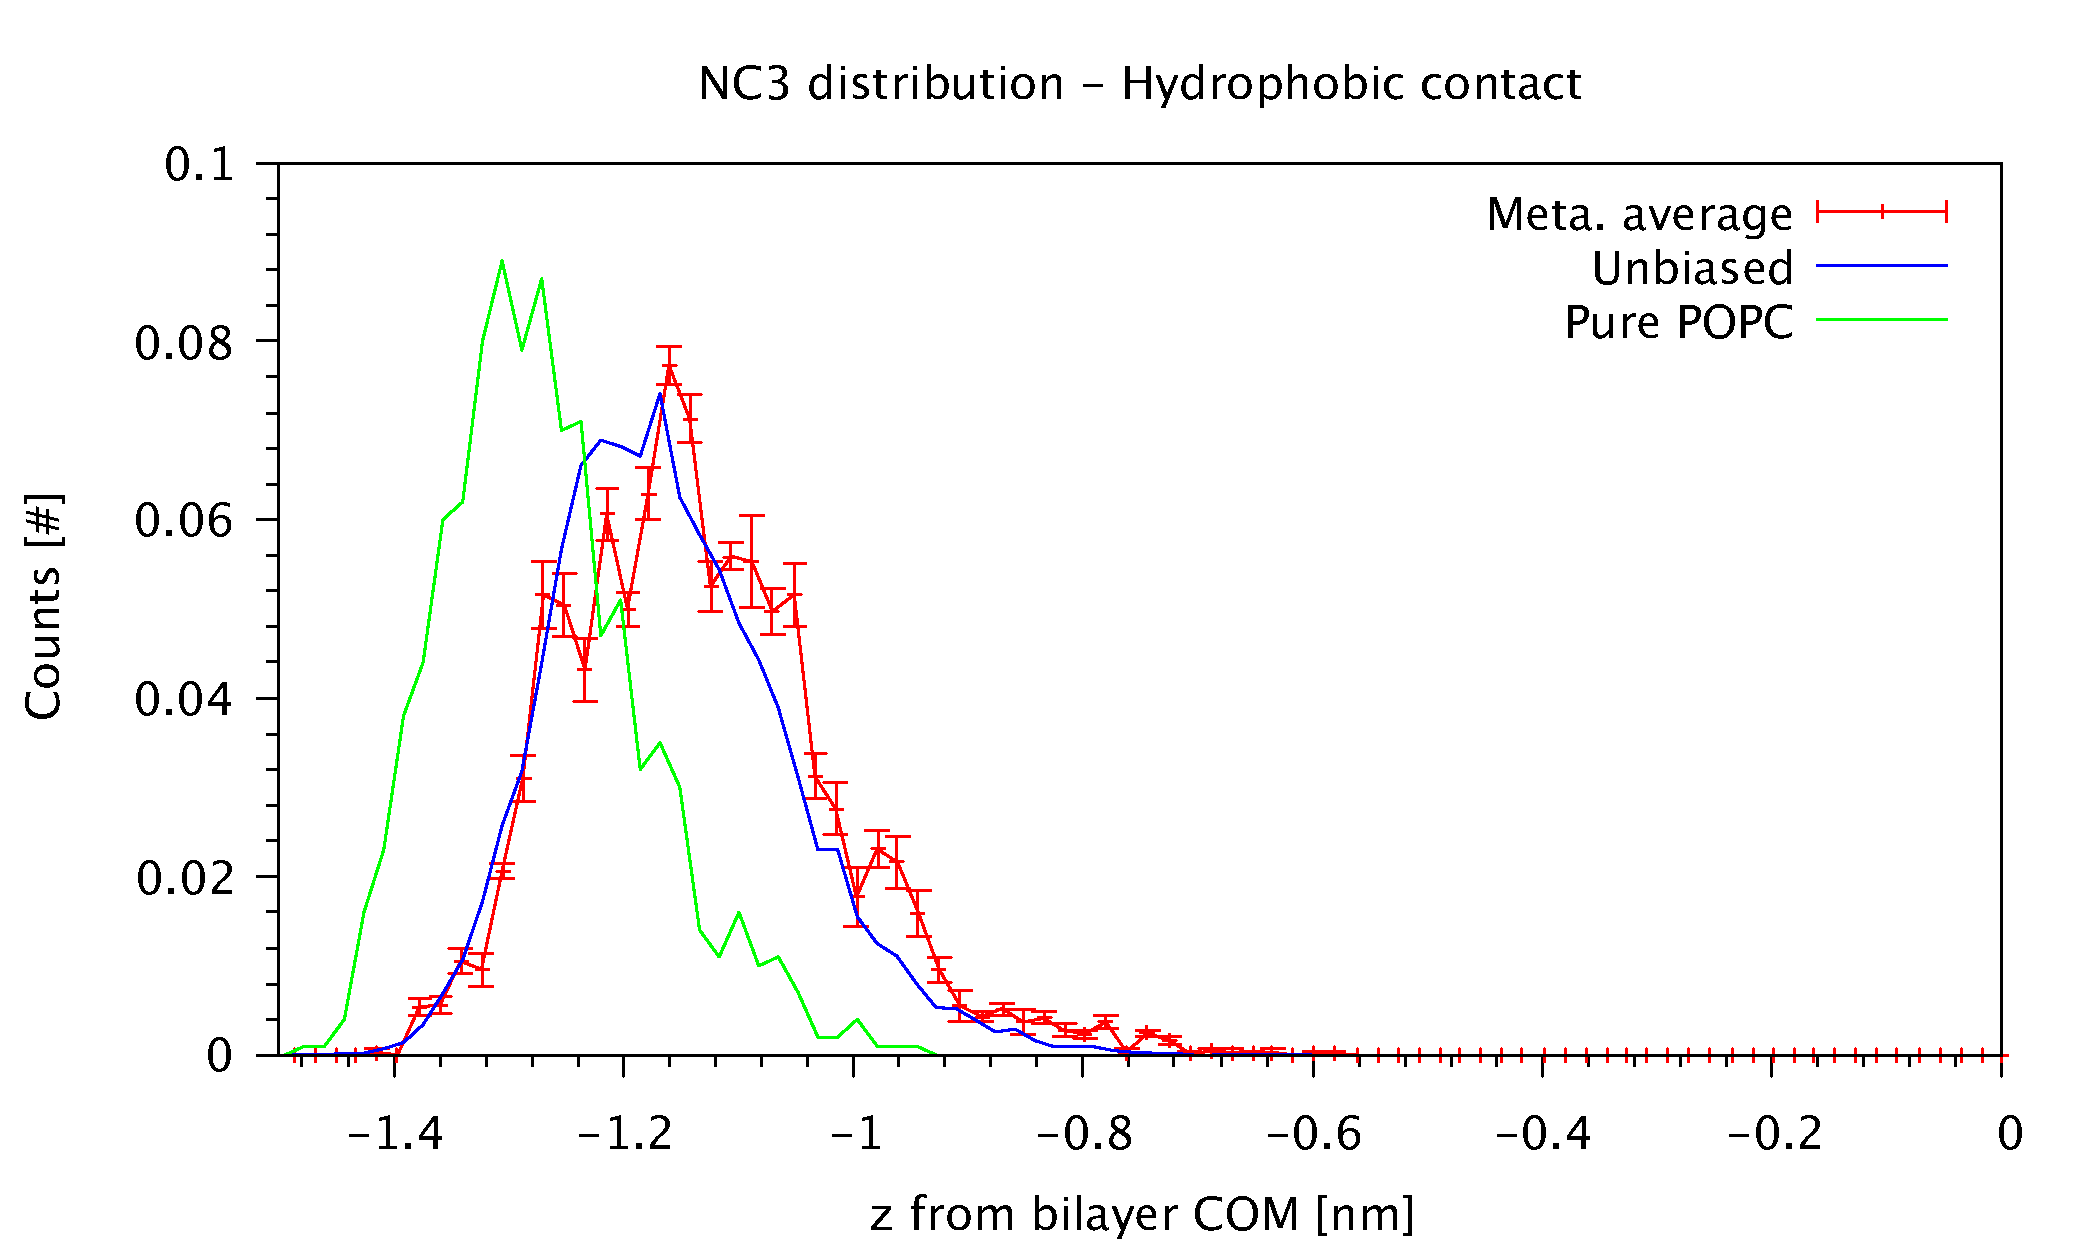
\includegraphics[width=0.95\textwidth]{./img/results/minDistHydroRandom11}
	}%
	\caption{Average distribution of the coline groups (NC3 beads) in the entrance leaflet closer to the bilayer \acs{COM} in function of the position of the charged bead in the hydrophobic state and in comparison with an average over ten metadynamics runs in the hydrophobic contact only, the unbiased run and a pure \acs{POPC} run for: (a) the striped \acs{NP}; (b) the random \acs{NP}.}
	\label{fig:NC3minDistUn}
\end{figure}

%	patchedPWContact	randon11PWContact
% 	patchedNC3Contact	random11NC3Contact
\begin{figure}[p]
	\center
	\begin{adjustwidth}{-0.5cm}{-1.5cm}
		\subfloat[striped NP]{
		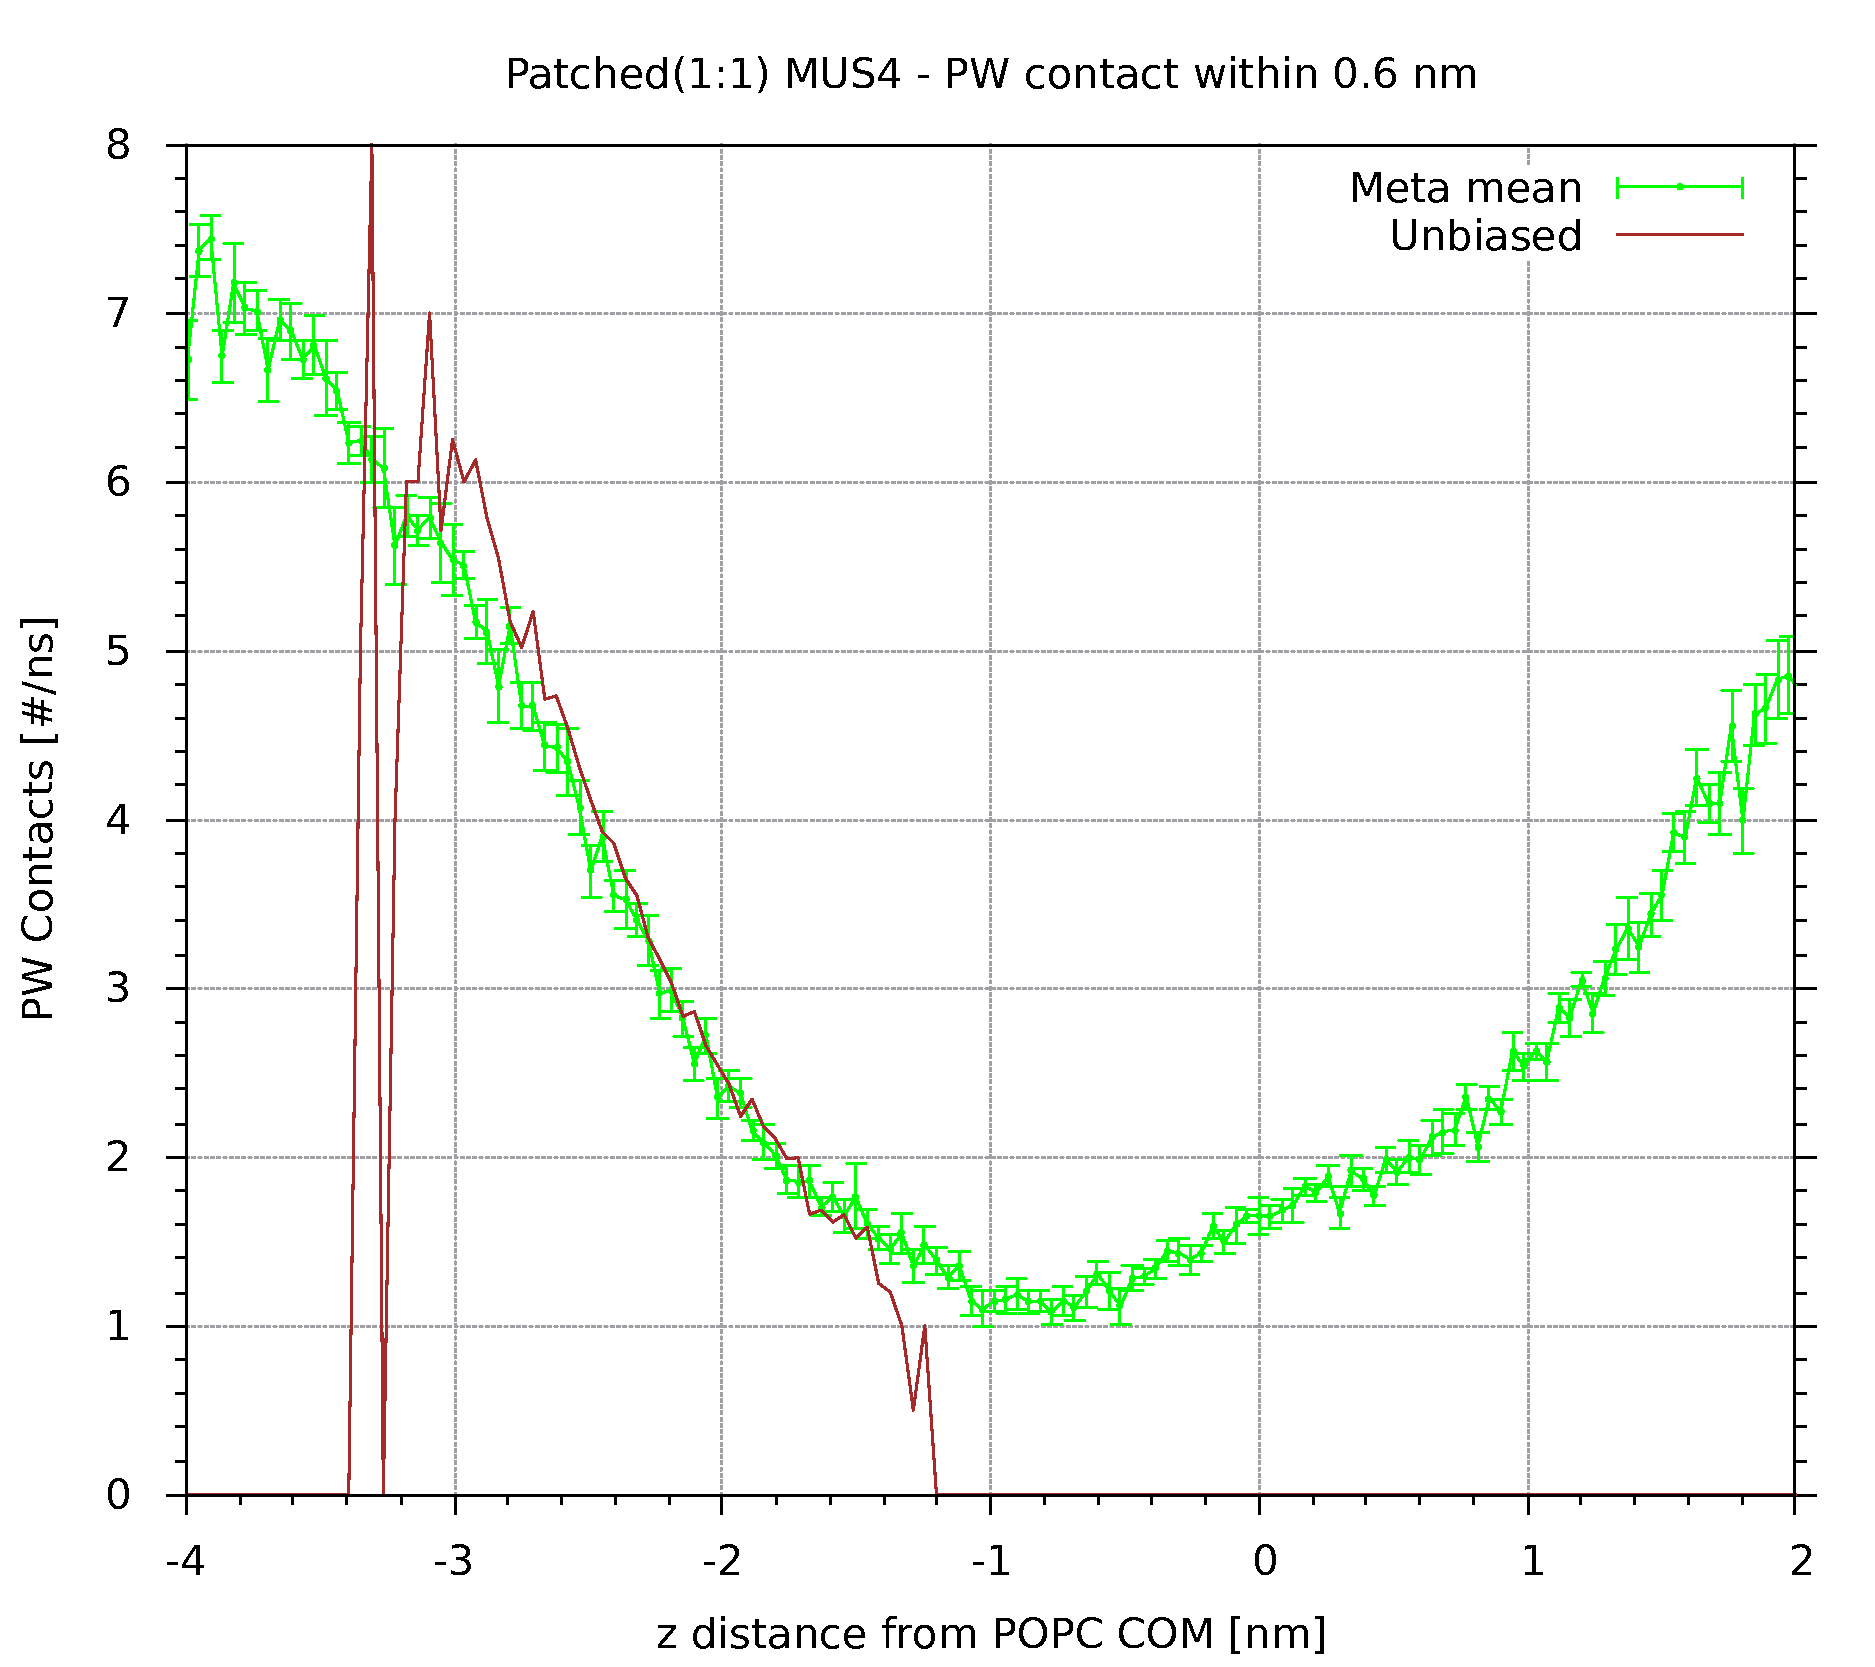
\includegraphics[width=0.5\linewidth]{./img/results/patchedPWContact}
		}%
		\subfloat[random NP]{
		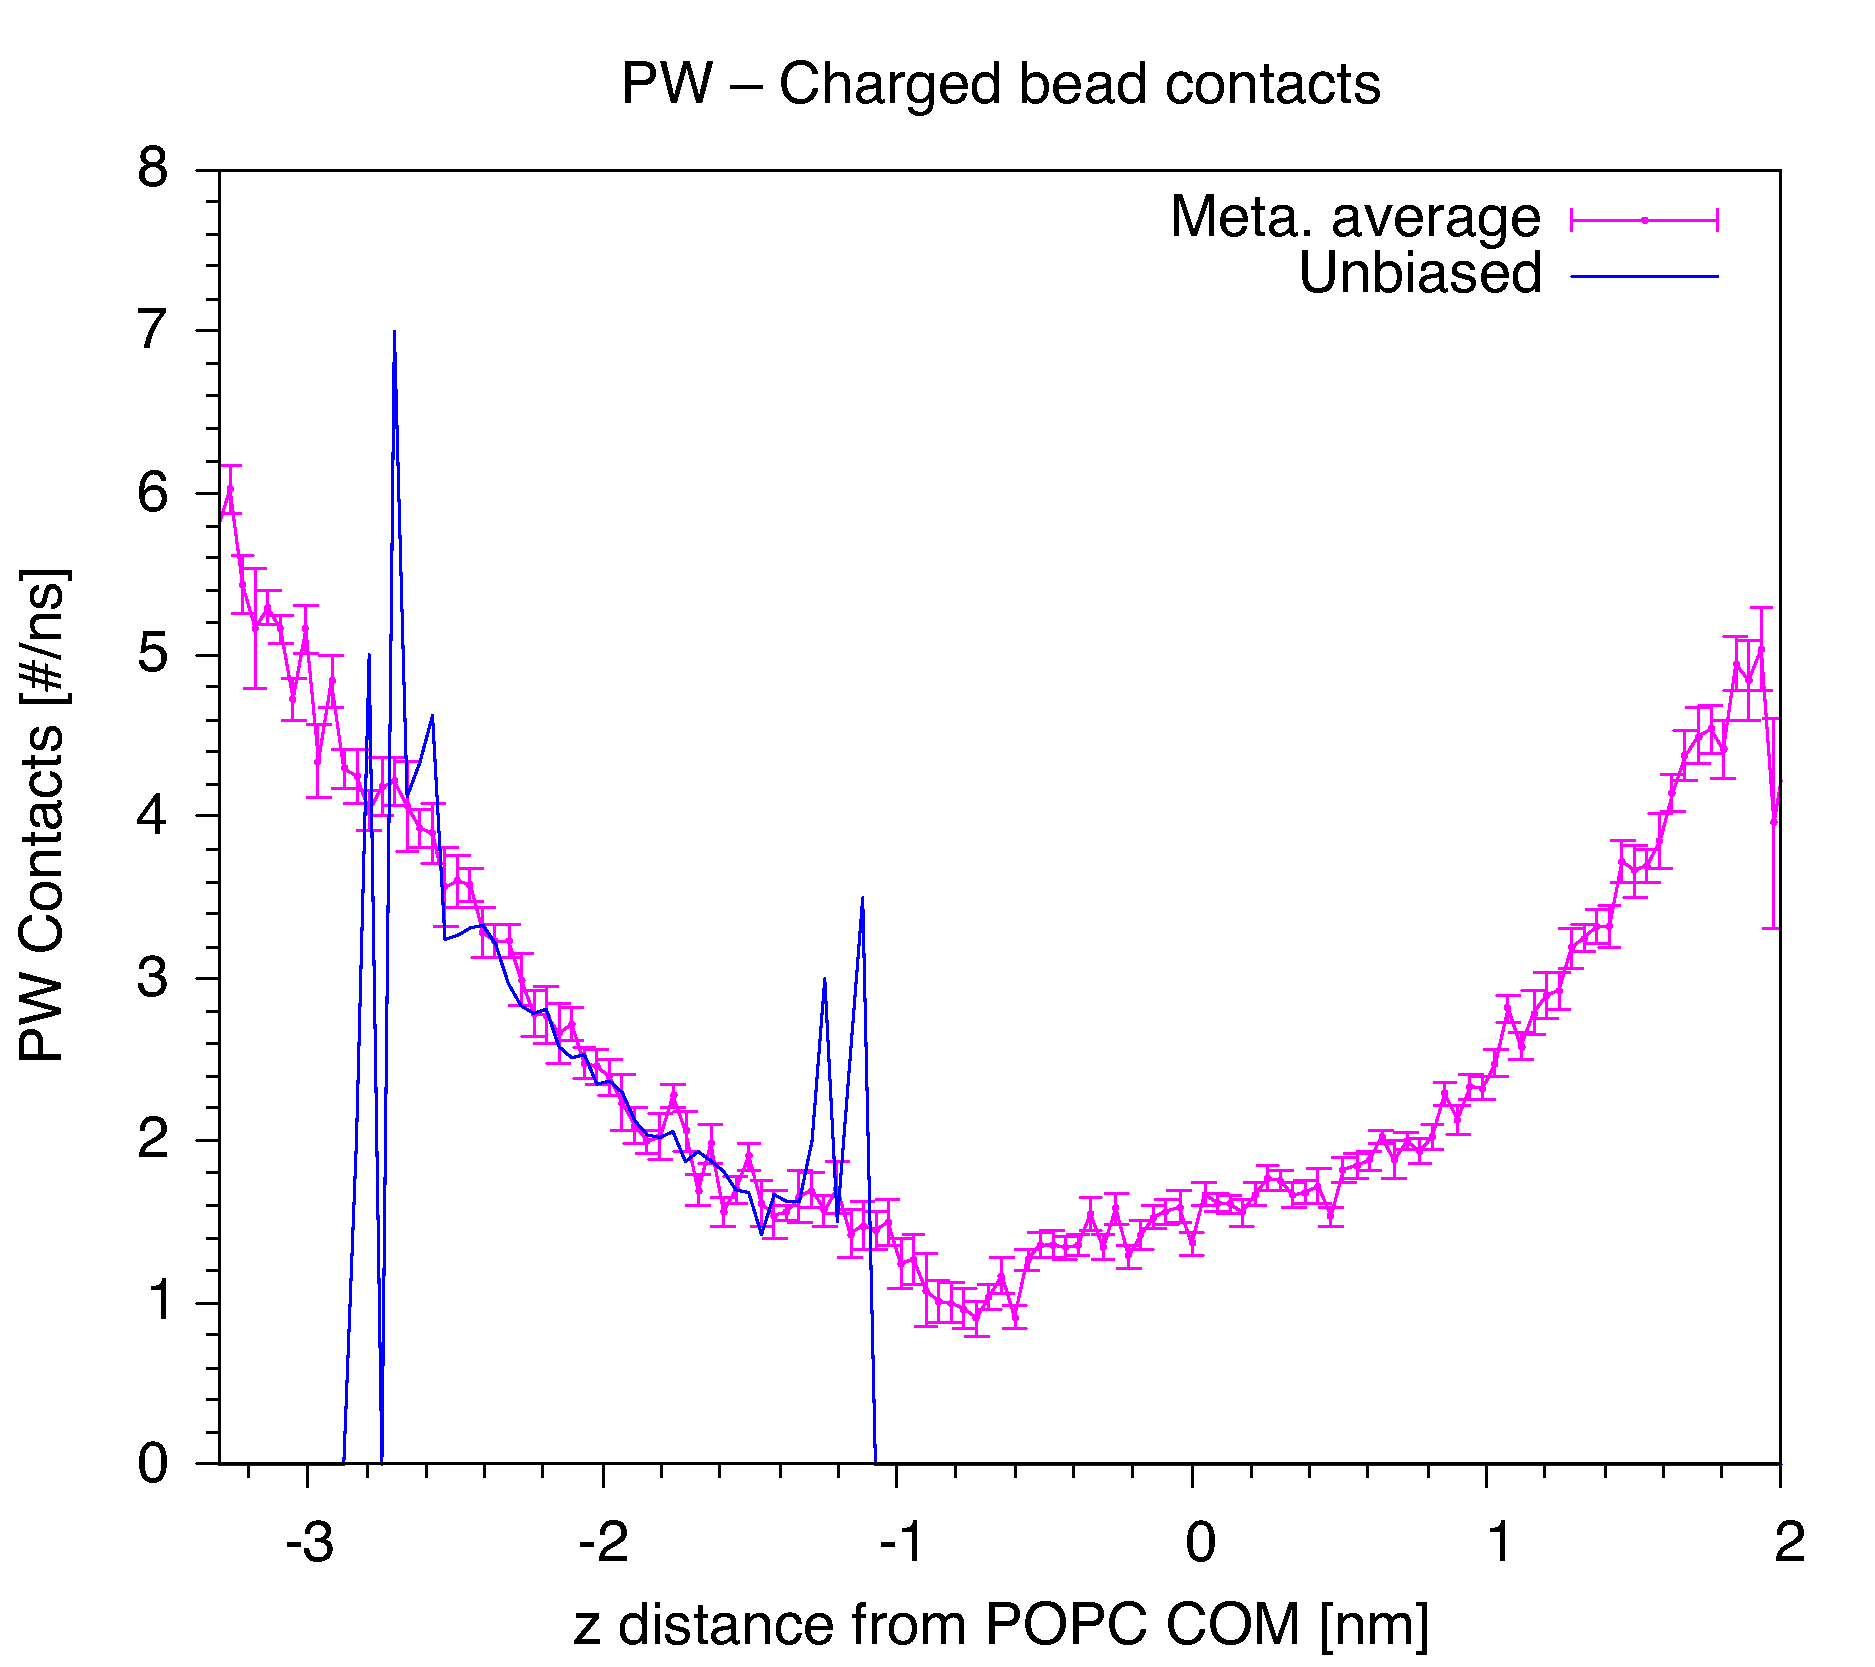
\includegraphics[width=0.5\linewidth]{./img/results/random11PWContact}
		}\\%
		\subfloat[striped NP]{
		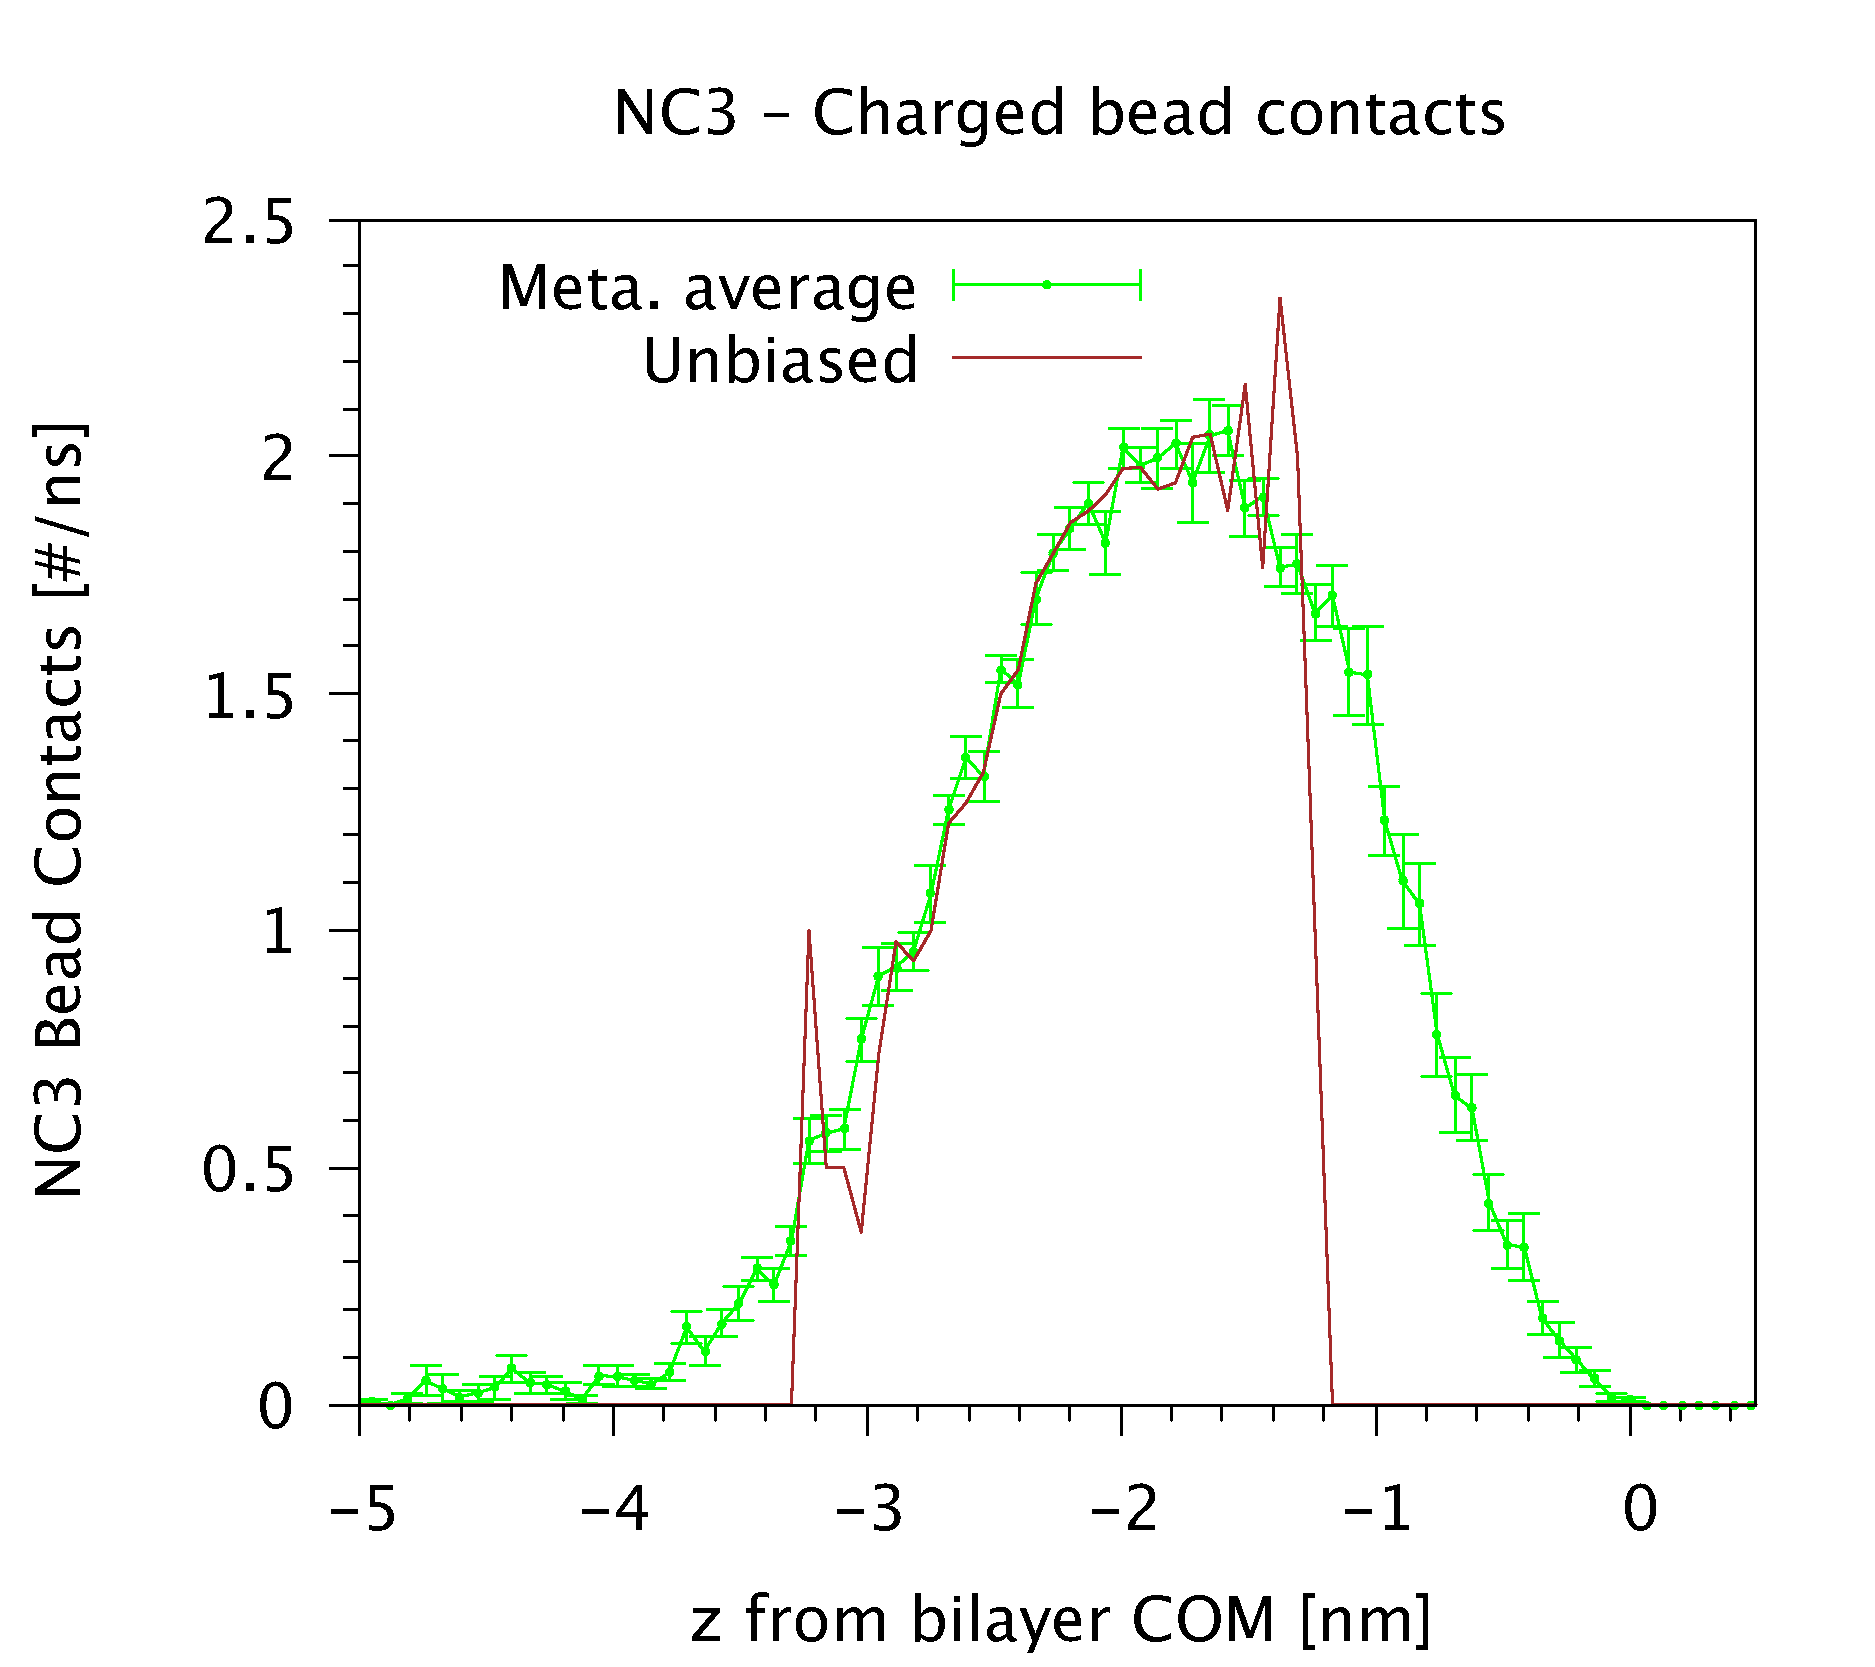
\includegraphics[width=0.5\linewidth]{./img/results/patchedNC3Contact}
		}%
		\subfloat[random NP]{
		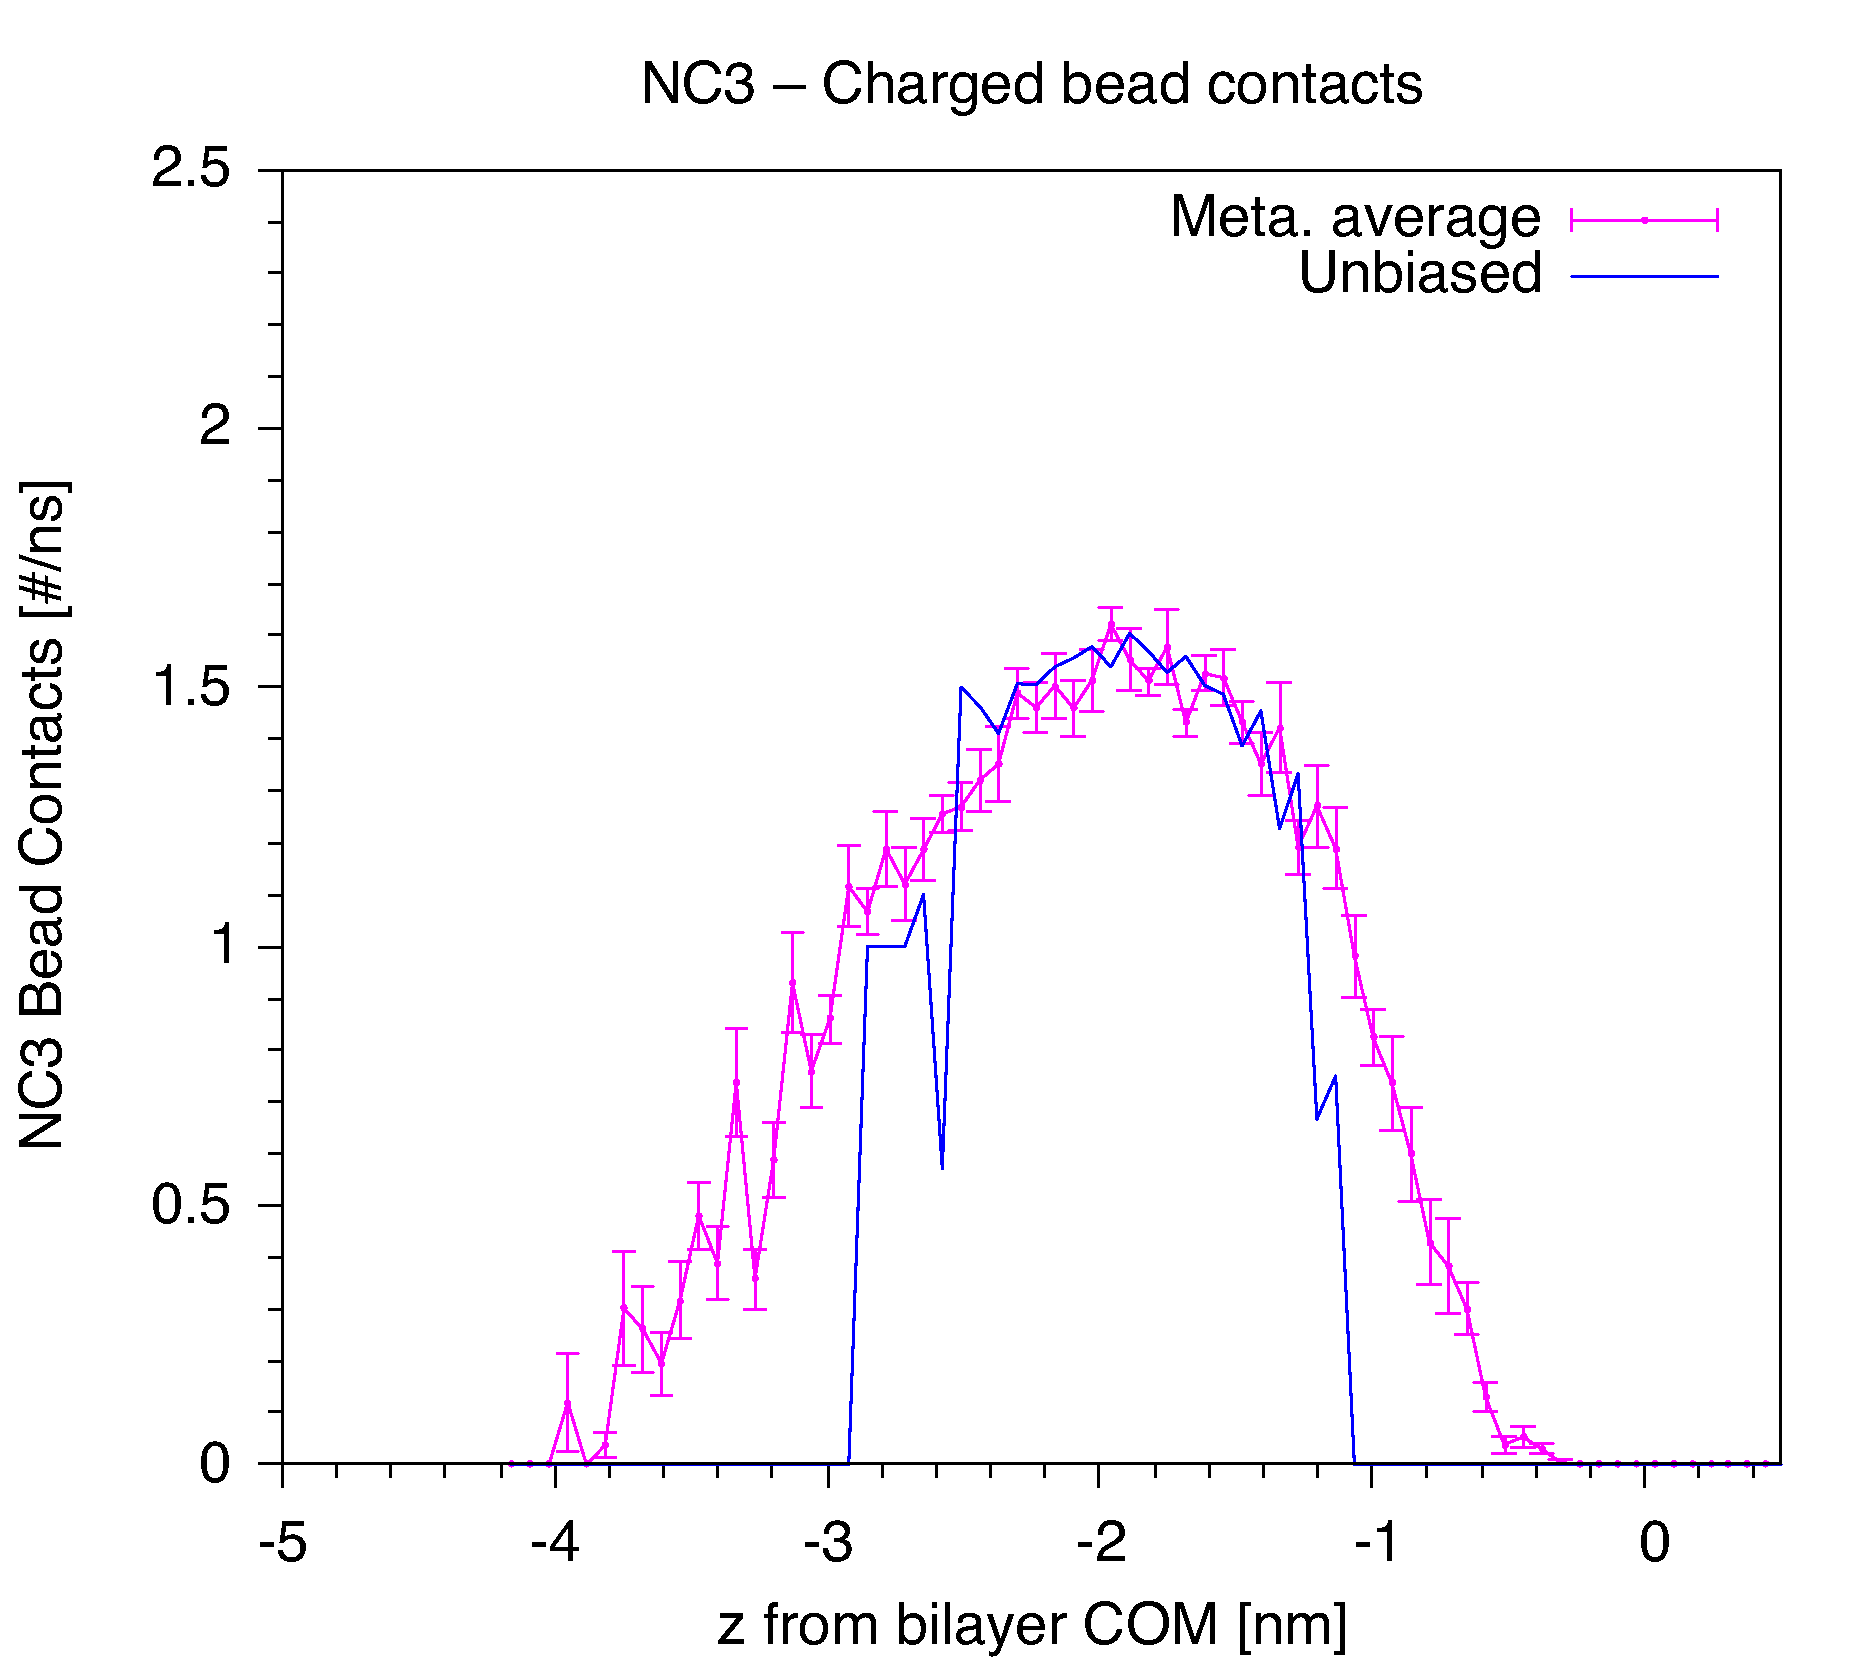
\includegraphics[width=0.5\linewidth]{./img/results/random11NC3Contact}
		}
		\caption{(a-b) Number of contacts per ns between the \acs{PW} beads and the charged bead in function of the position of the charged bead for: (a) the striped \acs{NP} and (b) the random \acs{NP}. (c-d) The same for the coline group and the charged bead  in the hydrophobic state for: (c) the striped \ac{NP} and (d) the random \acs{NP}. For each plots the number of contacts are in comparison with the corresponding unbiased runs.}
		\label{fig:contactsUn}
	\end{adjustwidth}
\end{figure}


\section{NP and membrane properties}
%Proprietà generali
%Coef di diffusione stato ancorato, stato idrofobico

\begin{table}[h!t]
	\centering
	\begin{tabular}{lccc}
		\toprule
		\,		& striped ($1$:$1$)		& random ($1$:$1$)		& random ($1$:$2$)		\\
		\,		& \acs{PW}$+$\acs{PME} & \acs{PW}$+$\acs{PME} & \acs{PW}$+$\acs{PME}	\\ \toprule
		$D^h_{\text{NP}}$ [$10^{-8}$~cm$^2$/s] & $12 \pm 2$ & $5 \pm 2$ & $5.7 \pm 0.7$ 			\\ \midrule
		$D_{tl}$ [$10^{-8}$~cm$^2$/s] & $30 \pm 1$ & $\mathbf{25 \pm 1}$ & $\mathbf{27.8 \pm 0.1}$	\\ \midrule
		$D_{bl}$ [$10^{-8}$~cm$^2$/s] & $\mathbf{22 \pm 2}$ & $27 \pm 3$	& $35 \pm 1$			\\ \midrule
		$\overline{d_z}$ [nm] & $1.996 \pm 0.0016$	& $2.2794 \pm 0.0017$	& $2.7284 \pm 0.0014$	\\ \bottomrule
	\end{tabular}
	\caption{Lateral diffusion coefficients: of the \acs{NP} in the hydrophobic state ($D^h_\text{NP}$), of the lipids in the top leaflet ($D_{tl}$) and in the bottom leaflet ($D_{bl}$). $\overline{d_z}$ is the average $z$ component of the distance between the \acs{COM} of the \acs{NP} and the \acs{COM} of the \acs{POPC} bilayer. The values in bold font refer to the entrance leaflet. Data obtained from my unbiased runs.}
	\label{tab:NPMembProperties}
\end{table}


\section{Structural properties of the bilayer}
%Risucchio delle membrane al recrossing
%Deformazione del leaflet di ancoraggio: RDF e densitymap 2D